{\documentclass[12pt,a4paper, spanish]{report}
\usepackage[spanish]{babel}
\usepackage[latin1]{inputenc}  % Ambos para solucin de asuntos de idioma
\usepackage[T1]{fontenc}
\usepackage{tocbibind}  % Bibliografa en el indice
\usepackage{titlesec}  % Posibilidad de editar los formatos de chapter y section
%\usepackage{times}  % Fuente de letras
\usepackage{amsmath,amssymb,mathrsfs,mathptmx}  % Matemticas varias
\usepackage{hyperref} % Para escribir URLs

\usepackage[]{algorithm2e}
\usepackage{listings}
% \usepackage{keyval,fancyvrb,xcolor,float,ifthen,calc,ifplatform}
% \usepackage{minted}



% --- Arreglos varios para la inclusion de imgenes
%\usepackage[pdftex]{graphicx}
%\usepackage[dvips]{graphicx}
\usepackage{graphicx}
\usepackage{epstopdf}
% \usepackage{epsfig}
\usepackage{float}
\usepackage{subfigure}
%\usepackage{subfig}
\usepackage{wrapfig}
\usepackage[usenames,dvipsnames]{color}
\DeclareGraphicsExtensions{.png,.jpg,.pdf,.mps,.gif,.bmp, .eps}


\usepackage{multirow}
\usepackage{multicol}
\usepackage{tabulary}
\usepackage[table]{xcolor}
\usepackage{color}
\usepackage{listings}
%\usepackage{subfloat}
\usepackage{tikz}

\setcounter{secnumdepth}{3}
\setcounter{tocdepth}{3}


% --- Para las dimensiones de los mrgenes etc
\frenchspacing \addtolength{\hoffset}{-1.5cm}
\addtolength{\textwidth}{3cm} \addtolength{\voffset}{-2.5cm}
\addtolength{\textheight}{4cm}
% --- Para el encabezado
\usepackage{fancyhdr}
\fancyhead[R]{2012}\fancyhead[L]{enCuadro} \fancyfoot[C]{\thepage}
\pagestyle{fancy}

% --- Formato de la etiqueta Chapter
%\newcommand{\bigrule}{\titlerule[0.5mm]}
%\titleformat{\chapter}[display]{\bfseries\Huge}
%{\Large\chaptertitlename\ \Large\thechapter}
%{0mm} {\filleft} [\vspace{0.5mm} \bigrule]

\titleformat{\chapter}[display]
{\normalfont\Large\filcenter}
{\titlerule[1pt]%
\vspace{1pt}%
\titlerule
\vspace{1pc}%
\LARGE\MakeUppercase{\chaptertitlename} \thechapter}
{1pc}
{\titlerule
\vspace{1pc}%
\Huge}

%-------------------------

\begin{document}
% Esto es para que se muestren todas las referencias aunque no se citen:
\nocite{*}

\renewcommand{\tablename}{Tabla}
\renewcommand{\theenumi}{\Roman{enumi}}
\renewcommand{\labelenumi}{[\textbf{\theenumi}]}
\renewcommand{\thefootnote}{\arabic{footnote}}
% --- Modificacin de entornos enumerate
\renewcommand{\theenumi}{\roman{enumi}}
\renewcommand{\labelenumi}{\theenumi)}
% --- Modificacin de entornos enumerate

% --- Para hacer highlights
\newcommand{\highlAmarillo}[1]{\colorbox{yellow}{#1}}
\newcommand{\highlVerde}[1]{\colorbox{green}{#1}}
\newcommand{\highlRojo}[1]{\colorbox{red}{#1}}



v0.2
\chapter{Detecci�n}
\label{ch:detection}

\section{Introducci�n}
En este cap�tulo se trata con algunas de las herramientas y algoritmos de detecci�n de caracter�sticas del tipo de primitivas geom�tricas como ser puntos, esquinas, bordes, l�neas, segmentos de l�nea y arcos. 

El objetivo principal es mostrar qu� caracter�sticas se pueden detectar y determinar qu� algoritmos son adecuados para su posterior utilizaci�n para la estimaci�n de pose, tema que se desarrolla en los Cap�tulos \ref{chap: camypose} y en forma m�s espec�fica en el Cap�tulo \ref{chap: posit}. El tipo de caracter�sticas elegidas para su detecci�n en la aplicaci�n final est�n fuertemente ligadas con el desempe�o del algoritmo que realiza dicha detecci�n. Existe un requerimiento de tiempo ya que la aplicaci�n final se debe ejecutar en tiempo real. Tambi�n se desea que la caracter�stica seleccionada ofrezca la posibilidad de ser procesada posteriormente mediante algoritmos relativamente simples.

Se busca que las caracter�sticas detectadas, asociadas a objetos o elementos presentes en la escena, presenten estabilidad en su ubicaci�n frente a cambios en la pose. En forma m�s espec�fica, si se tiene una esquina a detectar en una escena, por ejemplo de una mesa, la esquina puede ser detectada en im�genes o ``fotos'' de la mesa desde distintas posiciones y que en todos los casos la esquina detectada corresponde con la esquina de la mesa en la foto. Tambi�n se busca que las caracter�sticas sean robustas frente a cambios en las condiciones en que se adquiere la imagen. Estas condiciones podr�an ser iluminaci�n, presencia de ruido, oclusiones, etc.

El cap�tulo comienza con la revisi�n de algunos detectores cl�sicos de bordes y esquinas como son Canny y Harris. Posteriormente se desarrollan algunos detectores de l�neas, segmentos de l�nea y algunas estructuras m�s complejas, como el M�todo de la Transformada de Hough, LSD, EDLines y ORT. A lo largo de todo el cap�tulo se presentan resultados de estos algoritmos.
% \section{T�pos de caracter�sticas}

\section{Bordes y esquinas}
Los detectores de bordes, en particular los detectores de bordes tipo escal�n son una parte esencial de muchos sistemas de visi�n. El proceso de detecci�n de bordes cumple la funci�n de simplificar dr�sticamente la cantidad de informaci�n a procesar conservando aspectos estructurales utilizables para establecer los l�mites de cierto objeto en la imagen \cite{Canny:1986:ACA}. 

Un \textbf{borde} se puede definir intuitivamente como un cambio brusco sobre una zona en la intensidad de una imagen. M�s formalmente puede ser asociado a la b�squeda de discontinuidades y naturalmente su implementaci�n est� relacionada con la derivada primera de una imagen. En una imagen una derivada primera puede ser aproximada de distintas formas por un operador de gradiente como lo son los operadores de Sobel, Prewitt o Roberts por ejemplo\cite{operador_gradiente}. Hay implementaciones de detecci�n de bordes que toman en cuenta el \textit{efecto rampa} y por lo tanto acuden a derivadas de segundo y tercer orden. El efecto rampa se muestra en la Figura \ref{fig:rampa} en donde se puede ver en lo que aparentemente ocurre una discontinuidad en la imagen si uno se acerca lo suficiente a la regi�n, esta discontinuidad es en realidad continua.
\begin{figure}[h!]
  \centering
    
\includegraphics[scale=0.8]{figs_detection/rampa.png}
  \caption{Efecto rampa. A la izquierda una imagen que presenta una discontinuidad. A la derecha una acercamiento en la regi�n marcada en rojo.}
  \label{fig:rampa}
\end{figure}
	
\subsection{Detector de bordes de Canny}
El detector de bordes de Canny fue desarrollado en 1986 por John F. Canny \cite{Canny:1986:ACA} en el art�culo \emph{``A Computational Approach to Edge Detection''} con el objetivo de descubrir el algoritmo de detecci�n de bordes �ptimo. En esta secci�n se describe brevemente el algoritmo y se muestran algunos resultados de inter�s. La presentaci�n de este algoritmo est� inspirada principalmente en el art�culo del detector de bordes de Canny de Wikipedia \cite{canny_wiki}.\\ %\footnote{\url{http://en.wikipedia.org/wiki/Canny_edge_detector}}.

Las caracter�sticas buscadas por Canny para el detector de borde �ptimo son:
\begin{itemize}
 \item \textbf{Buena detecci�n}: El algoritmo debe marcar todos los bordes reales en la imagen como sea posible.
 \item \textbf{Buena localizaci�n}: Los bordes marcados deben estar lo m�s cercanos posibles a los bordes reales en la imagen.
 \item \textbf{Respuesta m�nima}: Dado un borde en la imagen este no debe ser marcado m�s de una vez y de ser posible la presencia de ruido no debe crear falsos bordes.
\end{itemize}
En la Figura \ref{fig:resultado_canny_lena}(b) se muestra un ejemplo del detector de bordes de Canny para la imagen de Lena original \ref{fig:resultado_canny_lena}(a).

\begin{figure}[h!]
  \centering
  \subfigure[Imagen de entrada: Lena]{
    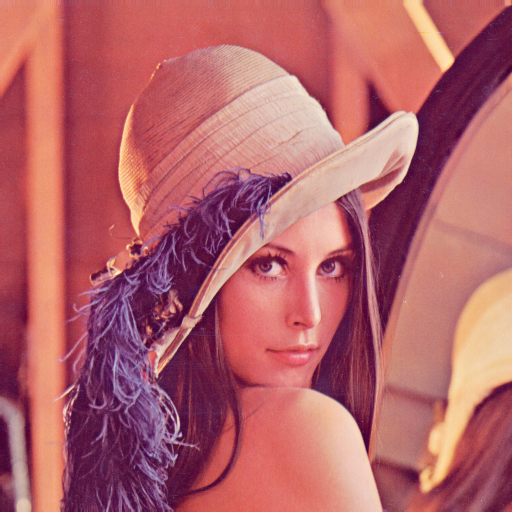
\includegraphics[scale=0.35]{figs_detection/canny/input_0.png}}
  \subfigure[Imagen de salida: Canny]{
    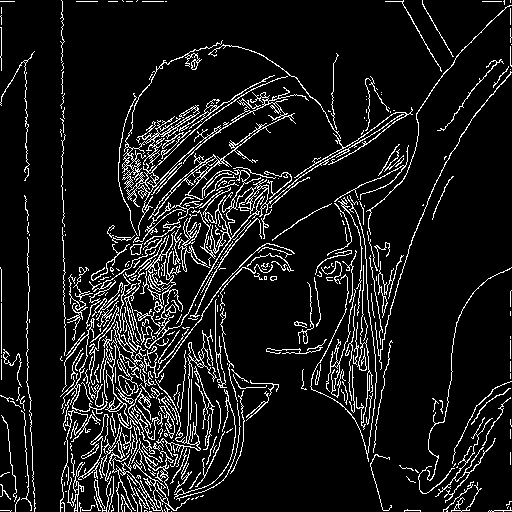
\includegraphics[scale=0.35]{figs_detection/canny/output.png}}
  \caption{Detector de bordes de Canny para la imagen Lena con par�metros: $\sigma=1.6$, $th_{lo}=4.0$, $th_{hi}=20.0$}
  \label{fig:resultado_canny_lena}
\end{figure}

El algoritmo consiste en cuatro etapas b�sicas las cuales se describen a continuaci�n. A lo largo de estas etapas se ejemplifica mediante el uso del demo \emph{online} de Canny en IPOL \cite{ipol_canny} para la imagen de Lena. Estos resultados intermedios se encuentran en la Figura \ref{fig:resultado_canny_lena_inter}.
\begin{itemize}

 \item 
\textbf{Reducci�n de Ruido}: Debido a que el detector de bordes de Canny es sensible a la presencia de ruido en las im�genes se utiliza en una primera etapa un filtrado Gaussiano en donde se realiza la convoluci�n de la imagen con un n�cleo Gaussiano. El resultado da lugar a una imagen levemente borrosa como se puede observar en la Figura \ref{fig:resultado_canny_lena_inter}(a).

 \item 
\textbf{Gradiente de intensidad de la imagen}: De forma de detectar bordes en todas las direcciones posibles, respecto a vecinos inmediatos de un p�xel, se utilizan cuatro filtros para detectar bordes en direcciones horizontal, vertical, y las dos direcciones diagonales. Un operador de detecci�n de bordes, por ejemplo Roberts, Prewitt o Sobel, devuelve un valor para la derivada primera en la direcci�n horizontal ($\mathbf{G}_x$) y otro para la derivada primera en la direcci�n vertical ($\mathbf{G}_y$). En base a estos valores se puede obtener m�dulo y direcci�n del gradiente sobre cada p�xel (Figura \ref{fig:resultado_canny_lena_inter}(b)). 
\begin{eqnarray}
\mathbf{G} = \sqrt{\mathbf{G}_x^2 + \mathbf{G}_y^2} \\
\Theta = \arctan\left(\frac{\mathbf{G}_y}{\mathbf{G}_x}\right)
\end{eqnarray}
Finalmente el �ngulo de direcci�n del borde es redondeado a uno de los cuatro �ngulos ($0$, $45$, $90$ o $135$ grados).

 \item 
\textbf{Supresi�n de no-m�ximos}: Dados los estimadores del gradiente de la imagen se realiza una b�squeda para determinar si el m�dulo del gradiente asume un rol de m�ximo local. De esta etapa se obtiene un conjunto puntos en forma de imagen binaria llamados \emph{``thin edges''} como se puede ver en la Figura \ref{fig:resultado_canny_lena_inter}(c). Estos proporcionan informaci�n de direcci�n para realizar el umbralizado con hist�resis.  

La b�squeda de m�ximos se realiza observando el �ngulo del punto y el m�dulo de �l y sus vecinos. Por ejemplo, si el �ngulo del gradiente pertenece al conjunto de los de cero grados (el borde es vertical) se observa el m�dulo de sus vecinos horizontales. Si el m�dulo del gradiente del punto es mayor a los de estos entonces el punto asume un rol de m�ximo local. Los otros casos son an�logos.

 \item 
\textbf{Umbrales con hist�resis}: El umbralizado con hist�resis requiere de dos umbrales, uno bajo y uno alto. El umbral alto asegura que se marcan bordes de los cuales se puede estar suficientemente seguros de que son borde (Figura \ref{fig:resultado_canny_lena_inter}(d)). Luego en base a los bordes correspondientes a umbrales altos se aplica el umbral bajo recorriendo los caminos de direcci�n obtenidos previamente. Una vez finalizado el proceso se tiene una imagen binaria en donde cada p�xel es marcado como borde o no (Figura \ref{fig:resultado_canny_lena_inter}(e)).
\end{itemize}

El algoritmo consiste en una serie de par�metros que ya fueron mencionados pero que vale la pena resaltar. En primer lugar el par�metro $\sigma$, la desviaci�n estandar del filtro Gaussiano utilizado en la etapa de reducci�n de ruido. Este par�metro afecta notablemente el desempe�o del algoritmo y debe ser ajustado seg�n la aplicaci�n ya que aporta un compromiso entre el detalle para bordes m�s fino y la cantidad de falsos bordes producto del ruido. Por otro lado en la etapa de umbralizado con hist�resis se tienen dos par�metros m�s, los valores de los dos umbrales; alto y bajo. En estos dos par�metros residen los t�picos problemas de los umbrales y no hay un enfoque gen�rico que lo solucione, si el umbral alto es muy alto se puede perder informaci�n importante y por otro lado si el umbral bajo es muy bajo se producir�n m�s falsos bordes debido a ruido. 
\begin{figure}[h!]
  \centering
  \subfigure[Reducci�n de ruido: Blur]{
    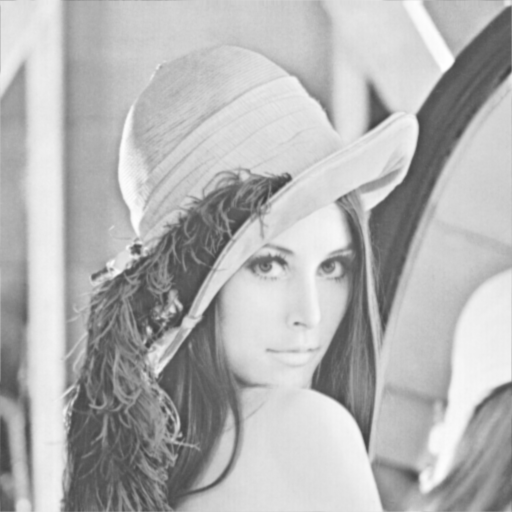
\includegraphics[scale=0.28]{figs_detection/canny/o_blur.png}}
  \subfigure[Gradiente]{
    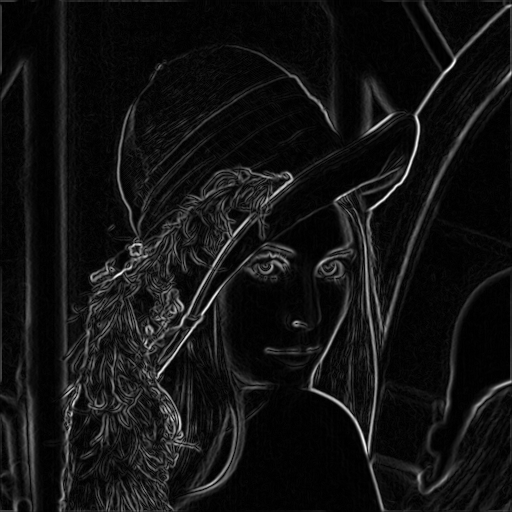
\includegraphics[scale=0.28]{figs_detection/canny/o_gradient.png}}
  \subfigure[Supresi�n de no-m�ximos]{
    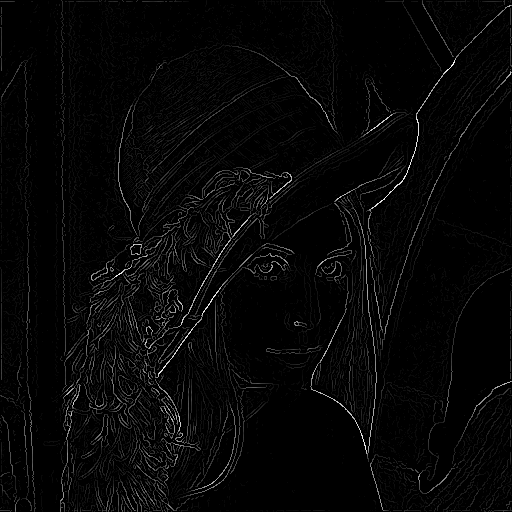
\includegraphics[scale=0.28]{figs_detection/canny/o_maxima.png}}
  \subfigure[Umbralizado con hist�resis: umbral alto]{
    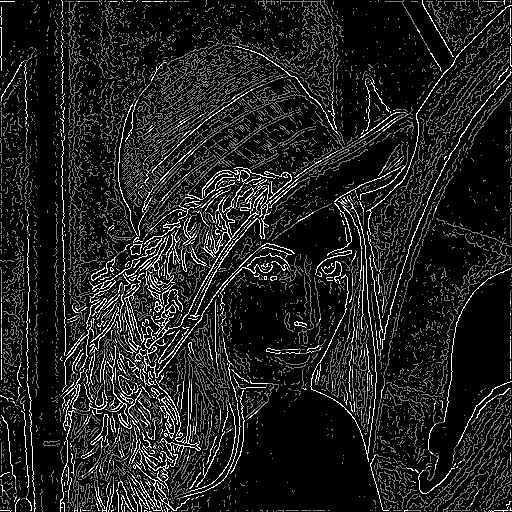
\includegraphics[scale=0.28]{figs_detection/canny/o_hi.png}}
  \subfigure[Umbralizado con hist�resis: umbral bajo]{
    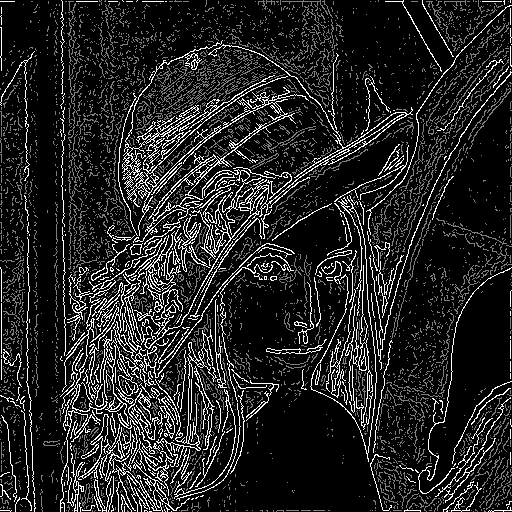
\includegraphics[scale=0.28]{figs_detection/canny/o_lo.png}}
  \caption{Resultados intermedios del detector de bordes de Canny para la imagen Lena con par�metros: $\sigma=1.6$, $th_{lo}=4.0$, $th_{hi}=20.0$}
  \label{fig:resultado_canny_lena_inter}
\end{figure}


\subsubsection{Ejemplos de inter�s}
En la Figura \ref{fig:resultado_canny_marcador} se muestran distintos resultados de Canny para distinto valor de $\sigma$, utilizando como entrada una imagen conteniendo el marcador utilizado en el proyecto.
\begin{figure}[h!]
  \centering
  \subfigure[Imagen de entrada: Marcador]{
    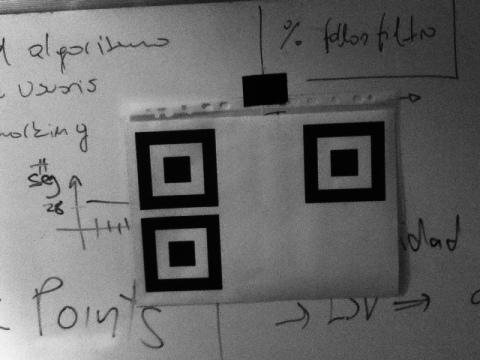
\includegraphics[scale=0.4]{figs_detection/canny_mrkr/canny_in.png}}
  \subfigure[$\sigma=0.5$]{
    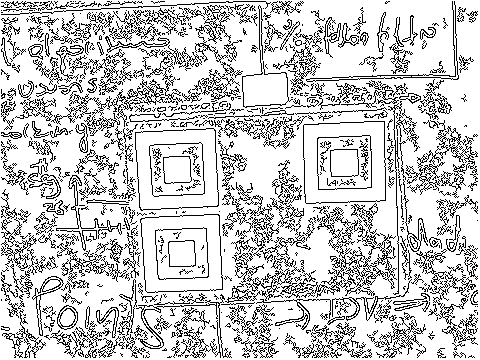
\includegraphics[scale=0.4]{figs_detection/canny_mrkr/canny_05.png}}
  \subfigure[$\sigma=1.4$]{
    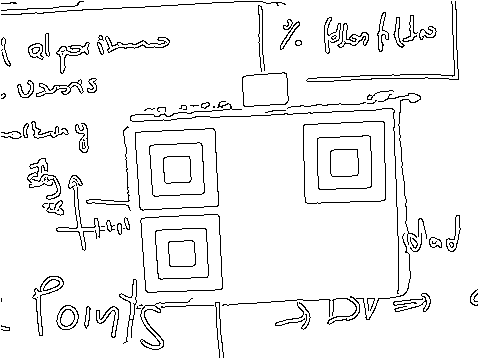
\includegraphics[scale=0.4]{figs_detection/canny_mrkr/canny_14.png}}
  \subfigure[$\sigma=6.0$]{
    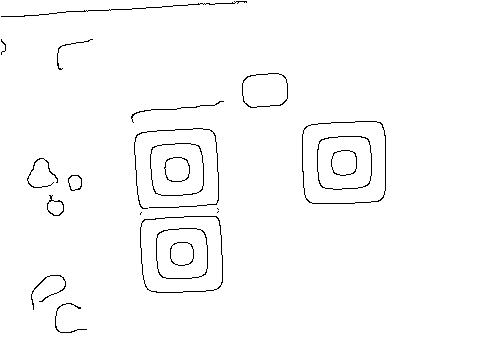
\includegraphics[scale=0.4]{figs_detection/canny_mrkr/canny_60.png}}
  \caption{Resultados del detector de bordes de Canny variando el par�metro de reducci�n de ruido $\sigma$ para una imagen de entrada conteniendo un marcador. $th_{lo}=0.2$, $th_{hi}=0.8$ (umbrales normalizados}
  \label{fig:resultado_canny_marcador}
\end{figure}
Se puede ver que con $\sigma = 0.5$ la presencia de ruido afecta notablemente la detecci�n produciendo una gran cantidad de falsos bordes. Para $\sigma=1.4$ la detecci�n es buena eliminando pr�cticamente todos los falsos bordes producto del ruido y conservando la informaci�n de borde real. Por otro lado para $\sigma=6.0$ el \emph{bluring} resulta en una detecci�n de bordes muy reducida aunque preservando la informaci�n de bordes m�s significativos como los bordes del marcador los cuales son el inter�s principal en la aplicaci�n. De todas formas se produce un efecto no deseado de ``redondeo'' de los bordes asociados al uso de un n�cleo Gaussiano circular.


\subsection{Detector de bordes y esquinas de Harris}
El detector de bordes y esquinas de Harris es un m�todo desarrollado por Chris Harris et al. en 1988 en el art�culo \emph{``A combined corner and edge detector''}\cite{Harris88acombined}. 

% Se considera una ventana en el p�xel $(x,y)$ en donde se define la suma
% cuadrada ponderada de los elementos de la ventana como
% $$E_{x,y}= \sum_{u,v} w_{u,v}[I_{x+u,y+v}-I(u,v)]^2 = \sum_{u,v} w_{u,v}[xI_x+yI_y+O(x^2,y^2)]^2 $$
% en donde $w_{u,v}$ es un n�cleo gaussiano para suavizar la respuesta y los gradientes pueden ser aproximados por
% $$I_x = I*(-1,0,1) \hspace{8mm} I_y = I*(-1,0,1)^T.$$
% Para peque�os variaciones, se puede tomar la aproximaci�n 
% $$E(x,y) = Ax^2 + 2Cxy + By^2$$
% en donde $A = I_x^2*w$, $B = I_y^2*w$ y $C = I_xI_y*w$. De forma de tomar en cuenta la variaci�n de $E$ junto con la direcci�n del cambio se reformula la
% ecuaci�n anterior como 
% $$E(x,y) =  \begin{pmatrix}
% 	      x &   y
% 	    \end{pmatrix}
% 		  \begin{pmatrix}
%                    A & C \\
% 		   C & B
%                   \end{pmatrix} \begin{pmatrix}
% 				    x\\
% 				    y
% 				\end{pmatrix} = \begin{pmatrix}
% 	      x &   y
% 	    \end{pmatrix}
% 		  M \begin{pmatrix}
% 				    x\\
% 				    y
% 				\end{pmatrix}$$
% Dado que $E$ est� fuertemente relacionado con la funci�n de autocorrelaci�n, si $\alpha$ y $\beta$ son los valores propios de la matriz $M$,
% ser�n proporcionales a la curvatura de la funci�n de autocorrelaci�n formando un descriptor invariante a rotaciones de $M$. La respuesta
% a esquinas propuesta para el detector de harris es computacionalmente m�s eficiente y no es necesario calcular valores propios de la matriz $M$. Esta dada
% por 
% $$R = det(M)-k tr^2(M)$$
% en donde $k$ es una constante de sensibilidad. Las esquinas est�n representadas por los valores de $R$ positivos mientras que los bordes corresponden a los 
% $R$ negativos y con $R$ cercano a cero tendremos zonas planas. 
Si tomamos una imagen $(I)$ en escala de grises y dos regiones solapadas de la misma que distan $(x,y)$ en las direcciones $i$ y $j$ respectivamente, definidas por una ventana $w(u,v)$; la suma ponderada del cuadrado de las diferencias entre ambas regiones ser\'a:\\
\[
E(x,y) = \sum_u{\sum_v{w(u,v) \left[ I(u+x,v+y) - I(u,v) \right]^2}}
\]
en donde $w_{u,v}$ es un n�cleo Gaussiano para suavizar la respuesta. Si realizamos una expansi\'on de Taylor de $I(u+x,v+y)$, obtenemos la siguiente aproximaci\'on:\\
\[
I(u+x,v+y) \approx I(u,v) + I_x(u,v)x + I_y(u,v)y
\]
Los gradientes de la imagen representados por $I_x$, $I_y$  pueden ser aproximados por:
$$I_x = I*(-1,0,1) \hspace{8mm} I_y = I*(-1,0,1)^T.$$
Reemplazando entonces:
\[
E(x,y) \approx \sum_u{\sum_v{w(u,v) \left[  I_x(u,v)x + I_y(u,v)y \right]^2}}
\]
o lo que es lo mismo:
\[
E(x,y) = ( \: x\:,\:y\: ) 
A 
\left(\begin{array}{c}
x\\
y
\end{array}\right)
\]
siendo:
\[
A = 
\left( 
\begin{array}{cc}
\left<I_x^2\right> & \left<I_xI_y\right> \\
\left<I_xI_y\right> & \left<I_y^2\right> 
\end{array} 
\right)
\]
donde los par\'entesis angulares denotan el promediado ponderado que puede ser, como se explica anteriormente, Gaussiano.\\

Por construcci\'on, es f\'acil ver que grandes variaciones en $E(x,y)$ ocasionadas por cambios en ambas direcciones $(i,j)$ estar\'an indicando la existencia de una esquina, mientras que grandes variaciones en $E(x,y)$ ocasionadas por cambios en una sola de direcci\'on indicar\'an la existencia de un borde. Es posible entonces limitar el estudio a la matriz A y sus valores propios.\\
Sean $\alpha$ y $\beta$ los valores propios de A. Se concluye por lo anterior que si:
\begin{itemize}
\item
Ambos valores propios son grandes: Se est� en presencia de una esquina.
\item
Un valor propio es grande y el otro peque\~no: Se est� en presencia de un borde.
\item
Ambos valores propios son peque\~nos: Se est� en presencia de una regi\'on ``plana''.
\end{itemize}
En la Figura \ref{fig:Fundamento1} se muestra la clasificaci�n de la regi�n correspondiente a la matriz $A$ correspondiente a las tres zonas de arriba. 
\begin{figure}[h!]
\centering
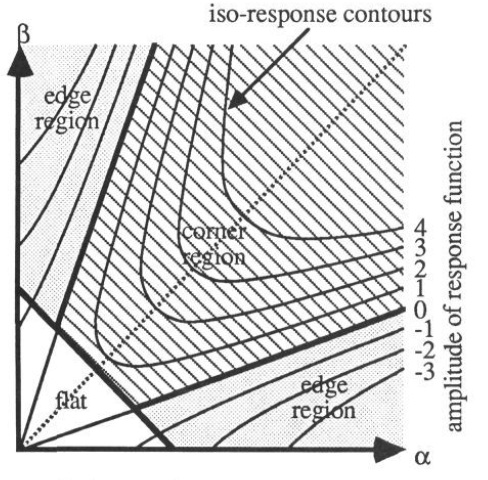
\includegraphics[scale=0.5]{figs_detection/harris/fundamento1.jpg}
\caption{Clasificaci�n de caracter�sticas seg�n los valores propios. Tomada de \cite{Harris88acombined}.}
\label{fig:Fundamento1}
\end{figure}
Debido a que el c�lculo de los valores propios de una matriz es un proceso computacionalmente costoso, se define la funci�n de respuesta $R$ que depende �nicamente de los valores propios $\alpha$ y $\beta$ y almacena b\'asicamente la misma informaci\'on.
\[
R = \alpha.\beta - k.(\alpha + \beta) = Det(A) - k.Tr(A)
\] 
donde $Det(A)$ denota el determinante de la matriz A, $Tr(A)$ su traza y $k$ es un par�metros de sensibilidad que normalmente pertenece al rango $[0.04 - 0.15]$. Por lo tanto se pueden clasificar los p�xeles de la siguiente forma:
\begin{itemize}
\item
$ R \gg 0$: Se tiene una esquina.
\item
$R \ll 0$: Se tiene un borde.
\item
$R \approx 0$: Se tiene una regi\'on ``plana''.
\end{itemize}

\subsubsection{Ejemplos de inter�s}
En la Figura \ref{fig:resultado_harris} se muestran los resultados para el detector de Harris provisto por Matlab en la funci�n \texttt{corner}. La misma tiene un par�metro modificable asociado a la m�xima cantidad de esquinas que se desean tener.
\begin{figure}[h!]
  \centering
  \subfigure[Harris para $n=50$]{
    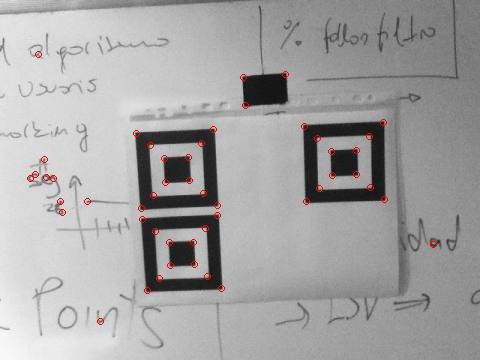
\includegraphics[scale=0.5]{figs_detection/harris/harris_50.png}}
  \subfigure[Harris para $n=100$]{
    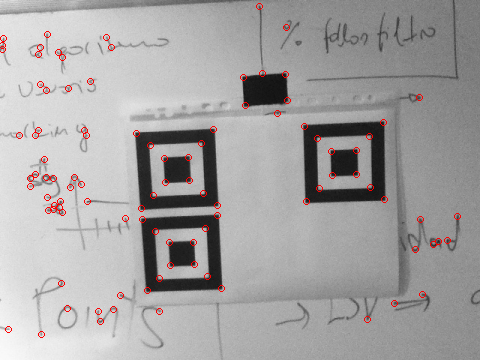
\includegraphics[scale=0.5]{figs_detection/harris/harris_100.png}}
  \caption{Resultados Harris para la imagen del marcaodor. El par�metro $n$ es un m�ximo en la cantidad de esquinas detectadas.}
  \label{fig:resultado_harris}
\end{figure}
Se puede ver que los resultados son buenos para ambos casos y particularmente buenos si se desean detectar las esquinas del marcador.

\subsubsection{Aplicabilidad}
Se pudo ver que el detector de Harris result� en una detecci�n razonable para el ejemplo tratado aunque su funcionamiento en general puede no ser tan bueno. Bajo otras condiciones menos controladas como para la detecci�n de esquinas naturales, no generadas por la presencia de un marcador, puede ser inestable y poco robusto requiriendo de alg�n tipo de validaci�n \emph{a posteriori}.

Una desventaja importante que tiene la detecci�n de caracter�sticas tipo esquinas es que si se desea saber qu� esquinas se unen entre s� mediante los lados del marcador sin ambiguedad se debe obtener m�s informaci�n que permita conectarlas. Por lo tanto un buen complemento puede ser el gradiente o una detecci�n de bordes. La detecci�n de l�neas o segmentos ya contiene esta informaci�n y por lo tanto parece m�s apropiada.

\section{L�neas y segmentos de l�nea}
Las l�neas o segmentos de l�nea son elementos que contienen una estructura m�s definida en comparaci�n con los bordes. Esta estructura definida produce a su vez que la detecci�n de este tipo de elementos sea m�s estable y menos sensible al ruido que la detecci�n de bordes o esquinas. Como se ver� en a lo largo de la secci�n, los detectores de l�neas que se presentan tienen en com�n que utilizan al inicio de la detecci�n las herramientas de gradientes y operadores gradientes o directamente la detecci�n de bordes en s� misma para realizar el objetivo de detecci�n de l�neas.

En esta secci�n de explican brevemente algunos detectores de l�neas y segmentos de l�nea. En primer lugar se menciona un detector de l�neas cl�sico y popular como es el detector de Hough y se explica su funcionamiento as� como sus principales desventajas que hacen que este m�todo sea descartado para su desarrollo en el proyecto. En segundo lugar se menciona y se hace referencia al cap�tulo en donde ser� tratado el detector de segmentos de l�nea, uno de los pilares principales de este proyecto, el LSD. Tambi�n se muestran otros detectores que fueron tomados en consideraci�n pero por diferentes razones (explicadas en su secciones correspondientes) no fueron utilizados como son el ORT y EDLines.

 \subsection{Detector de l�neas de Hough}
El M�todo de la Transformada de Hough forma parte de una t�cnica de extracci�n de caracter�sticas con fuerte aplicaci�n a detecci�n de curvas y l�neas. 

Esta t�cnica consiste en tres pasos b�sicos. En primer lugar la imagen en niveles de gris es procesada por un detector de bordes devolviendo una m�scara binaria en donde los puntos borde son marcados. En segundo lugar la Transformada de Hough es aplicada a la m�scara de forma de detectar candidatos a l�neas en forma de m�ximos locales. Esta transformada consiste en una representaci�n param�trica de formas geom�tricas. Para detecci�n de l�neas se utiliza la representaci�n
\begin{equation}
 r = xcos(\theta) + y sin(\theta)
\end{equation}
en donde $r$ representa la distancia entre la l�nea y el origen y $\theta$ es el �ngulo del vector perpendicular a la recta desde el origen. Es posible
asociar una recta al par de par�metros $(r, \theta)$. El plano $(r,\theta)$ es es plano de Hough. Se determina en este plano para cada punto de la imagen
una �nica sinusoidal en donde mediante su superposici�n se tendr�, para una serie de puntos alineados en la imagen, un punto de cruce de estas sinusoides dado
por los par�metros $(r,\theta)$. Mediante la b�squeda de m�ximos locales en el plano de Hough se tienen definidas l�neas en la imagen.

Finalmente los segmentos son extra�dos de las l�neas detectadas utilizando umbrales sobre dos par�metros geom�tricos: el largo m�nimo de un segmento y la distancia m�xima permitida entre dos segmentos consecutivos.\\

La principal desventaja del m�todo de la transformada de Hough para detecci�n de l�neas resulta ser el ajuste de par�metros. El detector de bordes contiene por lo menos un par�metro ajustable de tipo de sensibilidad, la Transformada de Hough est�ndar involucra usualmente cuatro par�metros. Uno asociado a la escala, un segundo asociado al compromiso entre falsos positivos y falsos negativos y los otros dos a la discretizaci�n de los par�metros $r$ y $\theta$, aunque estos �ltimos pueden ser asociados a la resoluci�n de la imagen. Por otro lado est�n los dos par�metros asociados a la etapa de extracci�n de segmentos \cite{GJMR08}.

El ajuste de estos par�metros puede dar problemas y desafortunadamente no hay una regla general para realizar esto. Si el ajuste es correcto este m�todo puede proveer muy buenos resultados pero en otro caso el desempe�o se puede ver fuertemente afectado.

\subsubsection{Ejemplos de inter�s}
En la Figura \ref{fig:resultado_hough} se muestran los resultados para el detector l�neas mediante el M�todo de la Transformada de Hough implementado por Matlab mediante el uso de la funci�n \texttt{houghlines}. El script utilizado se encuentra en el Centro de Documentaci�n de Mathworks\cite{matlab_hough}. Del script proporcionado se realizaron algunos cambios, se carg� la ruta de la imagen de entrada, se elimin� la rotaci�n a la imagen de entrada y se modificaron algunos par�metros. Los resultados mostrados representan los mejores casos para los distintos ajustes de par�metros probados. El tama�o m�nimo de segmento se fij� en $15$ y el m�ximo hueco entre segmentos a llenar en $8$.
\begin{figure}[h!]
  \centering
  \subfigure[El plano de Hough]{
    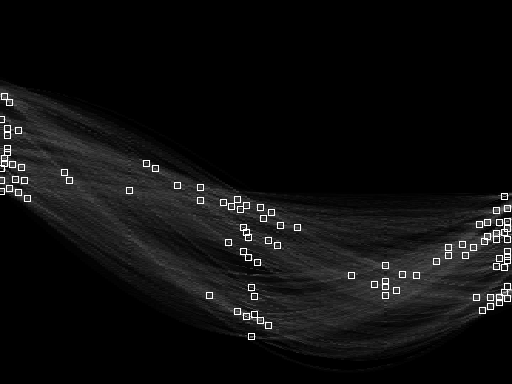
\includegraphics[scale=0.47]{figs_detection/hough/hough_transform.png}}
  \subfigure[Detecci�n de l�neas de Hough]{
    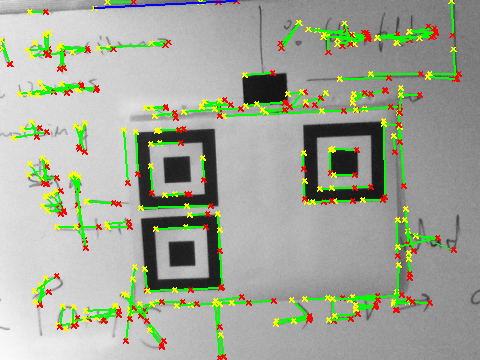
\includegraphics[scale=0.5]{figs_detection/hough/hough_lines.png}}
  \caption{Resultados para la detecci�n de l�neas por el M�todo de Hough para los par�metos: Tama�o m�nimo de segmentos $=15$, M�ximo hueco $=8$, N�mero de m�ximos $=100$ y Threshold en \texttt{houghpeaks} $=ceil(0.05*max(H(:)))$ }
  \label{fig:resultado_hough}
\end{figure}

\subsubsection{Aplicabilidad}
Se comprob� la dificultad intr�nseca del m�todo asociada al ajuste de par�metros no pudi�ndose obtener los resultados deseados en ning�n caso.

  \subsection{Detector de segmentos de l�nea: LSD}
El algoritmo Line Segment Detector (LSD) es capaz de detectar segmentos de l�nea rectos y uno de los componentes principales en este proyecto. Debido a su importancia es que se le dedica el Cap�tulo \ref{chap: lsd} a su desarrollo.

\subsubsection{Ejemplo de inter�s}
\begin{figure}[h!]
  \centering
    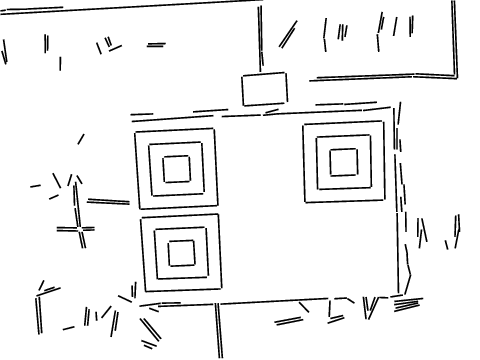
\includegraphics[scale=0.5]{figs_detection/lsd/lsd.png}
  \caption{Resultados de LSD para la imagen del marcador.}
  \label{fig:resultado_lsd_ipol}
\end{figure}
En la Figura \ref{fig:resultado_lsd_ipol} se muestran los resultados del algoritmo LSD para la imagen del marcador. Este ejemplo fue realizado mediante el uso del demo \emph{online} de IPOL para este algoritmo\cite{IpolLsd12}.

Se puede observar que el algoritmo logra detectar con �xito todas las estructuras de segmento de l�nea presentes en la imagen y en particular las que corresponden al marcador, los lados de los cuadril�teros.

El algoritmo produjo un n�mero de $169$ segmentos de l�nea detectados en un tiempo de ejecuci�n de $130ms$ sobre el servidor que aloja la aplicaci�n. La misma ejecuci�n realizada en el marco de este proyecto sobre una PC con procesador Intel Core 2 Duo de $2Ghz$ tom� un tiempo de aproximadamente $40ms$.

  \subsection{Detector de segmentos de l�nea: EDLines}
EDLines\cite{edlines} es un detector de segmentos de l�nea de tiempo lineal que provee resultados comparables con LSD. No requiere ajuste de par�metros y se ejecuta en tiempo real. En muchos aspectos es similar al LSD ya que utiliza validaci�n de l�neas mediante el principio de Helmholtz que permite controlar el n�mero de falsos positivos. El algoritmo hace uso del r�pido detector de bordes Edge Drawing (ED) \cite{edgedrawing} desarrollado por los mismos autores que provee una cadena de p�xeles borde en forma contigua.

EDLines trabaja sobre im�genes en niveles de gris y consiste b�sicamente en tres etapas: detecci�n de bordes seguido por extracci�n de segmentos y finalmente la validaci�n de l�neas. Se describen aqu� cada una de estas etapas.
\begin{itemize}
 \item 
\textbf{Detecci�n de bordes}: La detecci�n de bordes se realiza utilizando el algoritmo Edge Drawing el cual provee resultados r�pidos y libres de artefactos de ruido.

El algoritmo se aplica a la imagen de entrada en niveles de gris. En primer lugar se le aplica un filtrado para remoci�n de ruido y suavizar la imagen. A continuaci�n se calcula el gradiente, m�dulo y direcci�n, en cada pixel de la imagen suavizada. En tercer lugar se calculan un conjunto de p�xeles llamados \emph{anchors} que corresponden a puntos con alta probabilidad de ser borde. Por �ltimo se conectan estos \emph{anchors} mediante un proceso de dibujado de bordes entre ellos bas�ndose en el valor del m�dulo y direcci�n del gradiente previamente calculado. Este es en cierto sentido un proceso similar a los juegos de dibujo para ni�os.

 \item 
\textbf{Extracci�n de segmentos de l�nea}: El objetivo de esta etapa es el de ``partir'' la cadena contigua de p�xeles obtenida mediante el detector de bordes en uno o m�s segmentos de l�nea rectos. B�sicamente lo que se hace es recorrer la secuencia de p�xeles e ir ajustando l�neas a los p�xeles utilizando el m�todo de ajuste de l�neas por m�nimos cuadrados hasta que el error exceda cierto umbral. En el momento en que se excede ese umbral se genera un nuevo segmento de l�nea y as� recursivamente se recorren todos lo p�xeles de la cadena.

 \item 
\textbf{Validaci�n de l�neas}: El m�todo de validaci�n de segmentos de l�nea est� basado en el principio de Helmholtz el cual postula que para que una estructura sea perceptualmente significativa, la esperanza de que la misma (agrupado o Gestalt) ocurra de casualidad debe ser muy baja. Este es un efoque \emph{a contrario} en donde los objetos son detectados como \emph{outliers} sobre el modelo de fondo. En esta etapa se logra eliminar los falsos positivos controlando el n�mero de falsas alarmas. Este enfoque en particular es el propuesto originalmente por LSD y se explica tambi�n en el Cap�tulo \ref{chap: lsd}. 

Si la aplicaci�n lo permite, esta validaci�n puede ser eliminada o sustituida por otra, por ejemplo por un umbral de largo m�ximo de segmentos, acelerando a�n m�s el algoritmo EDLines. En LSD esta etapa esta integrada con la etapa de detecci�n de segmentos para cada iteraci�n aunque podr�a ser desacoplada en cierta medida. De todas formas EDLines presenta esa ventaja de modularidad frente a LSD que puede llegar a ser �til.
\end{itemize}

\subsection{Ejemplos de inter�s}
En la Figura \ref{fig:resultado_edlines}(a) se muestra la imagen de entrada junto con los segmentos detectados por EDLines para la imagen del marcador. En la Figura \ref{fig:resultado_edlines}(b) se muestra �nicamente los segmentos de salida de EDLines numerados.
\begin{figure}[h!]
  \centering
  \subfigure[Imagen de entrada y segmentos]{
    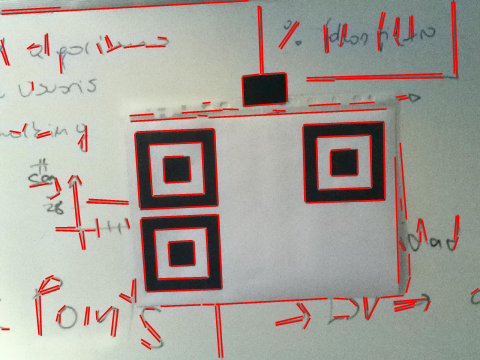
\includegraphics[scale=0.6]{figs_detection/edlines/edlines_img.png}}
  \subfigure[Segmentos de salida numerados]{
    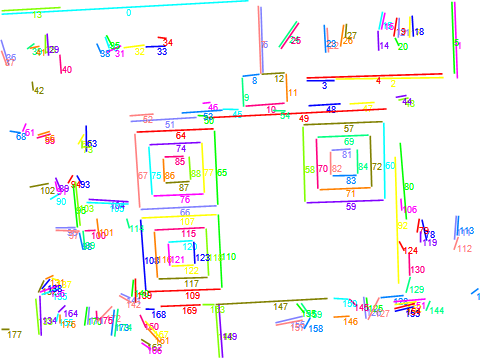
\includegraphics[scale=0.6]{figs_detection/edlines/edlines_nb.png}}
  \caption{Resultados de EDLines para la imagen del marcador.}
  \label{fig:resultado_edlines}
\end{figure}
El tiempo de ejecuci�n declarado para esta imagen por la aplicaci�n \emph{online} es de $30ms$ en su servidor pero alega que para una PC Intel con CPU de $2Ghz$ el mismo ser�a de $10ms$. Suponiendo una detecci�n en el tiempo declarado para una PC este ser�a dos veces m�s veloz que el de LSD para la misma imagen. Se detectaron $178$ segmentos y se puede ver que los resultados son muy similares a los que produce LSD que detecta $169$ segmentos para la misma imagen (Figura \ref{fig:resultado_lsd_ipol}).

\subsubsection{Aplicabilidad}
El algoritmo EDLines se encuentra disponible para descarga como una librer�a compilada para Windows o Linux. Tambi�n se puede probar en forma de demo \emph{online} desde la p�gina web del laboratorio Computer Vision \& Pattern Recognition de la Universidad de Anadolu de Turqu�a en donde tambi�n explica en forma resumida su funcionamiento\cite{edlines_demo}.\\

El c�digo fuente por su parte no est� disponible para la descarga de ning�n tipo en contraste con el LSD. Esto es un factor determinante para la utilizaci�n del algoritmo en el proyecto ya que se tiene que poder compilar para la plataforma de desarrollo utilizada, en este caso ser�a para el sistema operativo iOS. Una implementaci�n del algoritmo en lenguaje C/C++ no fue considerada como parte del alcance de este proyecto pero s� puede ser considerada como trabajo a futuro si se desea seguir con el enfoque de segmentos de l�nea para detecci�n.

  \subsection{Detector de segmentos de l�nea y arcos: ORT}
El Object Recongnition Toolkit (ORT) provee una serie de herramientas para la detecci�n de segmentos de l�nea, arcos y tambi�n puntos e incluso estructuras m�s complejas como pol�gonos. El c�digo est� disponible para su descarga en la p�gina del curso ``CSE 576 Computer Vision'' de la Univeristy of Washington de Estados Unidos de Am�rica\cite{ort_curso} como tambi�n desde un repositorio SVN p�blico se puede encontrar otra distribuci�n del c�digo con documentaci�n inclu�da\cite{ort_juanc}.

El ORT consiste en un n�mero de herramientas para ejecuci�n en cascada desde consola de comandos que resultan en la detecci�n de las caracter�sticas deseadas. Cada una de las herramientas corresponde a un algoritmo, estos son \textbf{Fex}\cite{fex}, \textbf{Lpeg}\cite{lpeg} e \textbf{Ipeg}. 

A continuaci�n de explican algunas de ellas.
\begin{itemize}

 \item 
\textbf{Chainpix}: produce una lista de p�xeles encadenados desde una imagen binaria que es salida de un detector de bordes tipo Canny. Se ejecuta mediante
\begin{verbatim}
chainpix < blocks.canny.pgm > blocks.cpx
\end{verbatim}
en donde \texttt{blocks.canny.pgm} es la imagen binaria salida de Canny y \texttt{blocks.cpx} la lista de p�xeles encadenados en un formato predefinido.

\item
\textbf{Fex}: convierte la lista de p�xeles encadenados en segmentos de l�nea rectos y arcos circulares. Su ejecuci�n se realiza mediante:
\begin{verbatim}
fex < blocks.cpx > blocks.fex
\end{verbatim}
y tiene como salida \texttt{blocks.fex}.

\item
\textbf{Lpeg}: realiza un agrupado de bajo nivel sobre los segmentos producidos por Fex hacia pares de l�neas paralelas y varios tipos de junturas. Tiene ciertos par�metros opcionales como el \emph{m�nimo largo de l�nea}, \emph{m�ximo �ngulo} tolerable entre dos l�neas paralelas y un \emph{nivel de calidad} m�nimo. Se ejecuta como:
\begin{verbatim}
lpeg < blocks.fex > blocks.lpg
\end{verbatim}
en donde la salida se escribe en \texttt{blocks.lpg}.

\item
\textbf{Ipeg}: realiza un agrupado de nivel medio sobre los conjuntos producidos por Lpeg hacia agrupaciones en tipo de ternas, esquinas y pol�gonos. Al igual que Lpeg tiene par�metros opcionales para producir �nicamente el tipo de agrupaciones de salida deseadas. Se ejecuta como:
\begin{verbatim}
ipeg < blocks.lpg > blocks.ipg
\end{verbatim}
en donde la salida se escribe en \texttt{blocks.ipg}.

\item
\textbf{Ort2Image}: toma la salida de Fex, Lpeg o Ipeg y realiza el dibujado de segmentos de l�nea rectos y segmentos de arco produciendo una imagen de salida en formato PGM.
\end{itemize}

\subsubsection{Ejemplos de inter�s}
En la Figura \ref{fig:resultado_ort} se muestran los resultados de las diferentes herramientas del ORT. Se utiliza como entrada el resultado del detector bordes de Canny para la imagen de la Figura \ref{fig:resultado_canny_marcador} para $\sigma = 1.4$ ya que fue el valor que demostr� mejores resultados entre las pruebas realizadas.
\begin{figure}[h!]
  \centering
  \subfigure[Imagen de entrada: Canny]{
    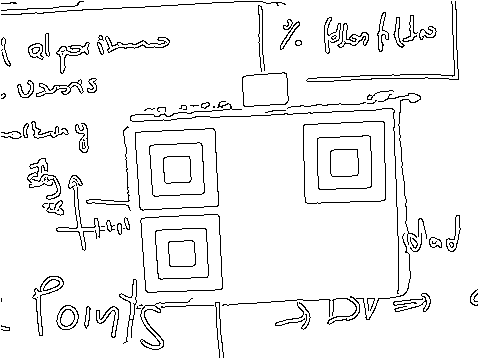
\includegraphics[scale=0.4]{figs_detection/ort/canny_140.png}}
  \subfigure[Fex]{
    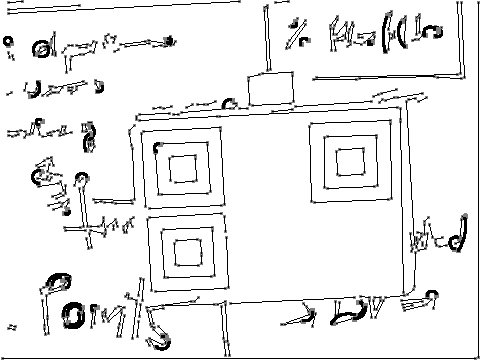
\includegraphics[scale=0.4]{figs_detection/ort/fex.png}}
  \subfigure[Lpeg]{
    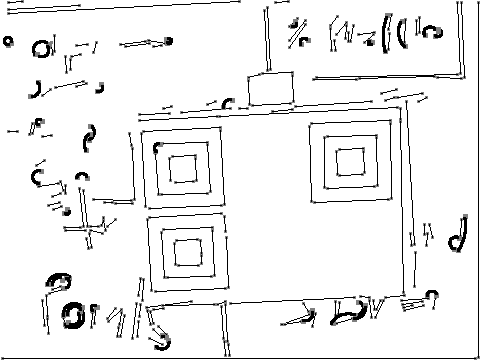
\includegraphics[scale=0.4]{figs_detection/ort/lpeg.png}}
  \subfigure[Ipeg]{
    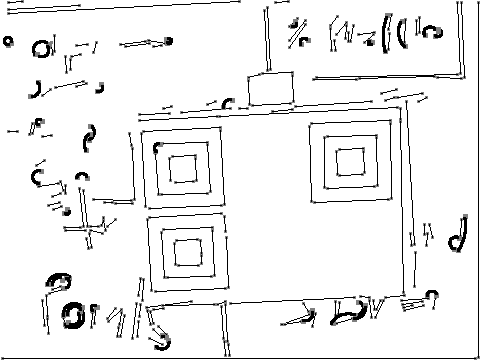
\includegraphics[scale=0.4]{figs_detection/ort/ipeg.png}}
  \caption{Resultados del Object Recognition Toolkit (ORT) para una imagen de entrada salida de Canny.}
  \label{fig:resultado_ort}
\end{figure}
Se puede observar que la salida de Fex logra capturar en buena forma los segmentos de l�nea correspondientes al marcador aunque alguno de ellos en forma ``quebrada''. Tambi�n se pueden ver los segmentos de arco detectados, otro de los elementos de este algoritmo. Lpeg logra eliminar una buena parte de los segmentos dejando s�lo aquellos que son en alg�n sentido paralelos entre s�. Por su parte Ipeg no produce ning�n cambio sobre los resultados de Lpeg. En otras pruebas realizadas tampoco se lograron los resultados deseados para este algoritmo a�n utilizando los par�metros opcionales. Un estudio m�s detallado del funcionamiento de esta herramienta en particular queda pendiente ya que resulta interesante para la aplicaci�n.

\subsubsection{Aplicabilidad}
El c�digo fuente de estas herramientas est� disponible para la descarga pero este genera un conjunto de programas ejecutables para consola de comandos. Su aplicaci�n para el proyecto no es directa ya que se deber�a portar a una interfaz compatible con nuestra aplicaci�n. Por otro lado mediante algunas pruebas realizadas sobre este algoritmo los tiempos de ejecuci�n total no resultaron suficientemente buenos para cumplir los requerimientos de tiempo real. Tambi�n se debe notar que aunque se obtuvieron resultados razonables para las herramientas Fex y Lpeg no fue as� para Ipeg que aporta un inter�s adicional para la aplicaci�n.

Un estudio m�s detallado del c�digo fuente y la posibilidad de reutilizarlo dentro del marco de la aplicaci�n queda como trabajo a futuro ya que ORT provee algunas herramientas interesantes y de m�s alto nivel que el detector de segmentos elegido LSD.

\section{Resumen}
En este cap�tulo se introdujo el tema de detecci�n de caracter�sticas orientado a primitivas. Se hizo �nfasis en el tipo de caracter�sticas de esquinas, bordes, l�neas y segmentos de l�nea recorriendo algunos algoritmos de detecci�n cl�sicos y otros m�s actuales. Se realiz� mediante el uso de un mismo ejemplo conteniendo un marcador algunas de las propiedades que interesan al proyecto concluyendo que el uso de segmentos de l�nea es el m�s apropiado por la naturaleza del marcador elegido. Se observ� que todos los algoritmos de l�neas y segmentos de l�nea analizados tienen en com�n la utilizaci�n de alg�n tipo de detecci�n de bordes o gradientes asociados a bordes al comienzo de la detecci�n. Se compararon los detectores de segmentos de l�nea obteniendo buenos resultados para los tres presentados, LSD, EDLines y ORT; eligiendo por diferentes razones LSD. A lo largo del an�lisis se establecieron pautas para realizar como trabajo a futuro en cuanto a los detectores de segmentos de l�nea, si es que se desea continuar con esta l�nea de trabajo.




\chapter{Marcadores}
\label{ch:marcadores}
\section{Introducci�n}
La inclusi�n de \emph{marcadores} en la escena ayuda al problema de extracci�n de caracter�sticas y por lo tanto al problema de estimaci�n de pose \cite{Lepetit05b}. Estos por construcci�n son elementos que presentan una detecci�n estable en la imagen para el tipo de caracter�stica que se desea extraer as� como medidas f�cilmente utilizables para la estimaci�n de la pose.

Los marcadores planos se pueden obtener mediante la construcci�n en una geometr�a coplanar de una serie de primitivas identificables como esquinas, segmentos o l�neas. Un �nico marcador plano puede contener por si solo todas las seis restricciones espaciales necesarias para definir un marco de coordenadas asociado a su pose.

Como se explica en el Cap�tulo \ref{chap: camypose} el problema de estimaci�n de pose requiere de una serie de correspondencias $\mathbf{M}_i\leftrightarrow \mathbf{m}_i$ entre puntos 3D en la escena en coordenadas del mundo y puntos en la imagen.

En el primer lugar se explican brevemente algunos de los sistemas de Realidad Aumentada m�s populares basados en marcadores planos. En segundo lugar se propone el dise�o de un marcador espec�fico para la aplicaci�n a este proyecto y se desarrollan las soluciones a los algoritmos de detecci�n de dicho marcador mostrando algunos resultados parciales en el proceso. Por �ltimo se muestran algunos resultados de Benchmark para establecer l�mites para la detecci�n.

\section{Sistemas basados en marcadores planos}
Existen muchos sistemas de visi�n basados en \emph{marcadores planos} con aplicaci�n en Realidad Aumentada y Navegaci�n. Algunos de ellos son \emph{ARToolKit}
 \cite{artoolkit}, \emph{ARTag} \cite{artag} y \emph{ARToolKitPlus} \cite{artoolkitplus} utilizados para Realidad Aumentada. A continuaci�n se realiza una breve descripci�n del funcionamiento general de los mismos.

Los sistemas basados en marcadores planos utilizan t�picamente marcadores bitonales. Esto perimte reducir la sensibilidad a las condiciones de luz de la escena y a las configuraciones de la c�mara por lo que no hay necesidad de identificar tonos de grises y la regla de decisi�n para cada p�xel puede ser reducida, en la versi�n m�s simple, a un umbral o \emph{threshold} \cite{markerdetection}. El dise�o de los marcadores depende en gran medida de la aplicaci�n. En la figura \ref{fig:Marcadores_AR} se muestran algunos marcadores planos para aplicaciones de Realidad Aumentada en donde cada uno de ellos provee suficientes puntos para permitir el c�lculo de pose tridimensional y adicionalmente contienen cierta informaci�n en su interior para permitir su identificaci�n.
\begin{figure}[h!]
  \centering
  \subfigure[\emph{ARToolKit}]{
    
\includegraphics[scale=0.45]{figs_detection/artoolkit.png}}
  \subfigure[\emph{ARTag}]{
    
\includegraphics[scale=0.45]{figs_detection/artag.png}}
  \caption{Cuatro ejemplos de marcadores para los sistemas de Realidad Aumentada indicados. Figura tomada de \cite{artag}.}
  \label{fig:Marcadores_AR}
\end{figure}

Es importante que los marcadores puedan ser localizados en un campo de visi�n amplio para permitir la correcta detecci�n bajo la distorsi�n asociada a la transformaci�n proyectiva que lleva el marcador en el mundo real al plano de imagen. Por otro lado, si los marcadores contienen informaci�n en su interior, esta no debe ser muy densa para permitir la recuperaci�n de la misma a mayor distancia. T�picamente, esta informaci�n es solo una identificaci�n entre marcadores de un mismo sistema por lo que la informaci�n es poca y esto no es un problema.

Estos sistemas contienen ciertos puntos caracter�sticos con los que se realiza el c�lculo de pose. En general su contorno es basado en un cuadril�tero y se utilizan las cuatro esquinas del contorno del marcador para realizar el c�lculo. 

Si se utiliza un �nico marcador la cantidad de puntos necesarios para la estimaci�n de pose resultan ser pocos lo que puede ser una desventaja en cuanto a la precisi�n del algoritmo de estimaci�n de pose. Esto se puede mejorar construyendo un marcador m�s complejo compuesto de una serie de marcadores y mediante la identificaci�n de los mismos asignar los puntos correspondientes para la estimaci�n de pose.

\subsection{ARToolKit}
\emph{ARToolKit} es un muy popular sistema de marcadores planos para Realidad Aumentada e Interacci�n Hombre-Computador. Su popularidad reside ser de los primeros proyectos en utilizar la Realidad Aumentada en dispositivos m�viles y tambi�n debido a que es un proyecto de c�digo abierto. 

Los marcadores bitonales consisten en un cuadrado con borde negro y un patr�n en el interior. La primer etapa del proceso de reconocimiento consisten en detectar los bordes negros. Esto se realiza buscando grupos conexos de p�xeles (\emph{blobs}) que est�n por debajo de un determinado umbral. Posteriormente se extrae el contorno de cada grupo, esos grupos que est�n rodeados por cuatro l�neas rectas son marcados como marcadores potenciales. Las cuatro esquinas de cada marcador potencial son utilizados para calcular la homograf�a y as� remover la distorsi�n perspectiva. Con el marcador en una vista can�nica, se procede a identificar el patr�n interno muestreando en una grilla, de por lo general $16\times 16$ o $32\times 32$, los valores de gris. Con esto se construye un vector caracter�stico y se compara por correlaci�n con una librer�a de vectores de caracter�sticos logrando la identificaci�n del mismo.

Este sistema tiene algunas desventajas o ``puntos d�biles''. En primer lugar la detecci�n es basada en un umbral por lo que las condiciones de iluminaci�n pueden afectar fuertemente la efectividad de la misma. Dado que el c�digo esta disponible este se puede modificar para realizar \emph{threshold} local o adaptivo por ejemplo. Otras desventajas est�n relacionadas con el proceso de identificaci�n del marcador frente a la librer�a.

\subsection{ARTag}
\emph{ARTag} es otro sistema de marcadores planos para Realidad Aumentada e Interacci�n Hombre-Computador que surge como una evoluci�n de ciertos aspectos de \emph{ARToolKit}. Los marcadores son tambi�n bitonales y basados en un borde negro. En contraste con el \emph{ARToolKit} este sistema utiliza un enfoque basado en bordes por lo que es m�s robusto a condiciones de iluminaci�n. Los bordes son unidos en segmentos que a su vez se unen en cuadril�teros. Al igual que con \emph{ARToolKit} con las esquinas se calcula la homograf�a y se muestrea en el interior del marcador pero con una grilla de $6\times 6$. 

El sistema puede lidiar con condiciones de iluminaci�n cambiantes, oclusiones y segmentos partidos hasta cierto punto. Otra mejora notable con respecto a \emph{ARToolKit} reside en el sistema de identificaci�n de marcadores. El proceso de identificaci�n de los marcadores entre s� es a su vez m�s veloz y robusto que el de \emph{ARToolKit}.

\section{Marcador QR}
El enfoque elegido para la detecci�n de caracter�sticas utilizando marcadores parte del trabajo de fin de curso denominado Autoposicionamiento 3D de \emph{Mat�as Tailani�n} y \emph{Santiago Paternain} para el curso \emph{Tratamiento de im�genes por computadora} de Facultad de Ingenier�a, Universidad de la Rep�blica\cite{tailanian}. La elecci�n se basa principalmente en los buenos resultados obtenidos para dicho trabajo con un enfoque relativamente simple. El trabajo desarrolla, entre otras cosas, un dise�o de marcador y un sistema de detecci�n de marcadores basado en el detector de segmentos LSD \cite{GJMR08} por su buena \emph{performance}. 

El marcador utilizado est� basado en la estructura de detecci�n incluida en los c�digos \emph{QR} y se muestra en la Figura \ref{fig:Marker}. �ste consiste en tres grupos id�nticos de tres cuadrados conc�ntricos superpuestos en ``capas''. La primer capa contiene el cuadrado negro de mayor tama�o, en la segunda capa se ubica el cuadrado mediano en color blanco y en la �ltima capa un cuadrado negro peque�o. De esta forma se logra un fuerte contraste en los lados de cada uno de los cuadrados facilitando la detecci�n de bordes o l�neas. El resultado de una detecci�n de l�neas para esta configuraci�n produce para cada cuadrado la detecci�n de sus lados. A diferencia de los c�digos \emph{QR} la disposici�n espacial de los grupos de cuadrados es distinta para evitar ambig�edades en la identificaci�n de los mismos entre s�. 
% Estas dos caracter�sticas son esenciales para la extracci�n de los \emph{puntos fiduciales} de forma coherente, es decir, las correspondencias tienen que poder ser determinadas completamente bajo criterios razonables.
\begin{figure}[h!]
\centering

\includegraphics[scale=0.3]{figs_detection/Marker.eps}
\caption{Marcador propuesto basado en la estructura de detecci�n de c�digos QR.}
\label{fig:Marker}
\end{figure}

\subsection{Estructura del marcador}
\label{sec:detection_estructuras}
A continuaci�n se presentan algunas definiciones de las estructuras b�sicas que componen el marcador propuesto. Estas son de utilidad para el dise�o y forman un flujo natural y escalable para el desarrollo del algoritmo de determinaci�n de correspondencias.\\

Los elementos m�s b�sicos en la estructura son los \emph{segmentos} los cuales consisten en un par de puntos en la imagen, $\mathbf{p} = (p_x,p_y)$ y $\mathbf{q} = (q_x,q_y)$. Estos \emph{segmentos} forman lo que son los lados del \emph{cuadril�tero}, el pr�ximo elemento estructural del marcador.\\

Un \emph{cuadril�tero} o \emph{quadrilateral} en ingl�s, al que se le denomina $Ql$, est� determinado por cuatro segmentos conexos y distintos entre s�. El cuadril�tero tiene dos propiedades notables; el \emph{centro} definido como el punto medio entre sus cuatro v�rtices y el \emph{per�metro} definido como la suma de el largo de sus cuatro lados. Los \emph{v�rtices} de un cuadril�tero se determinan mediante la intersecci�n, en sentido amplio, de dos segmentos contiguos. Es decir, si $s_1$ es contiguo a $s_2$ dadas las recta $r_1$ que pasa por los puntos $(\mathbf{p}_1$, $\mathbf{q}_1)$ del segmento $s_1$ y la recta $r_2$ que pasa por los puntos $(\mathbf{p}_2, \mathbf{q}_2)$ del segmento $s_2$, se determina el v�rtice correspondiente como la intersecci�n $r_1 \cap r_2$. \\
%La propiedad de conexi�n entre dos segmentos se relaja a la intersecci�n de dos discos de un cierto radio en torno a los puntos de dos segmentos vecinos. \\

A un \emph{conjunto de cuadril�teros} o \emph{quadrilateral set} se le denomina $QlSet$ y se construye a partir de $M$ cuadril�teros, con $M>1$. Los cuadril�teros comparten un mismo centro pero se diferencian en un factor de escala. A partir de dichos cuadril�teros se construye un lista ordenada $(Ql[0],Ql[1],\dots,Ql[M-1])$ en donde el orden viene dado por el valor de per�metro de cada $Ql$. Se define el \emph{centro del grupo de cuadril�teros}, $\mathbf{c}_i$, como el promedio de los centros de cada $Ql$ de la lista ordenada.\\

Finalmente el \emph{marcador QR} est� constituido por $N$ conjuntos de cuadril�teros dispuestos en una geometr�a particular. Esta geometr�a permite la determinaci�n de un sistema de coordenadas; un origen y dos ejes a utilizar. Se tiene una lista ordenada  $(QlSet[0],QlSet[1],\dots,QlSet[N-1])$ en donde el orden se puede determinar mediante la disposici�n espacial de los mismos o a partir de hip�tesis razonables.\\

Un marcador proveer� un numero de $4\times M \times N $ v�rtices y por lo tanto la misma cantidad de puntos para proveer las correspondencias $\mathbf{M}_i\leftrightarrow \mathbf{m}_i$ al algoritmo de estimaci�n de pose. De esta forma se tienen una cantidad de puntos superior a los que se podr�an tener utilizando uno de los marcadores de los sistemas como \emph{ARToolKit} a un costo de detecci�n relativamente bajo. Por otro lado se podr�a agregar alg�n patr�n para la identificaci�n de marcadores en la esquina que completa el rect�ngulo en donde no hay $QlSet$ como se realiz� en el trabajo Autoposicionamiento 3D \cite{tailanian}.

\subsection{Dise�o}
En base a las estructuras previamente definidas es que se describe el dise�o del marcador. Como ya se explic� se toma un marcador tipo QR basado en cuadril�teros y m�s espec�ficamente en tres conjuntos de tres cuadrados dispuestos en como se muestra en la figura \ref{fig:Marker}.\\

Los tres cuadril�teros correspondientes a un mismo conjunto de cuadril�teros tienen id�ntica alineaci�n e id�ntico centro. Los diferencia un factor de escala, esto es, $Ql[0]$ tiene lado $l$ mientras que $Ql[1]$ y $Ql[2]$ tienen lado $2l$ y $3l$ respectivamente. Esto se puede ver en la figura \ref{fig:QlSetDetail}. Adicionalmente se define un sistema de coordenadas con centro en el centro del $QlSet$ y ejes definidos como $\textbf{x}$ horizontal a la derecha e $\textbf{y}$ vertical hacia abajo. Esta convenci�n en las direcciones de los ejes es muy utilizada en el �rea de Procesamiento de Im�genes para definir las direcciones de los ejes de una imagen. Definido el sistema de coordenadas se puede fijar un orden a los v�rtices $v_{j_{1}}$ de cada cuadril�tero $Ql[j]$ como,
\begin{align*}
v_{j_{0}} = (a/2,a/2) && v_{j_{2}} = (-a/2,-a/2)  \\
v_{j_{1}} = (a/2,-a/2)&& v_{j_{3}} = (-a/2,a/2)
\end{align*}
con $a=(j+1)\times l$. El orden aqu� explicado se puede ver tambi�n junto con el sistema de coordenadas en la figura \ref{fig:MarkerDetail}.\\
\begin{figure}[h!]
\centering
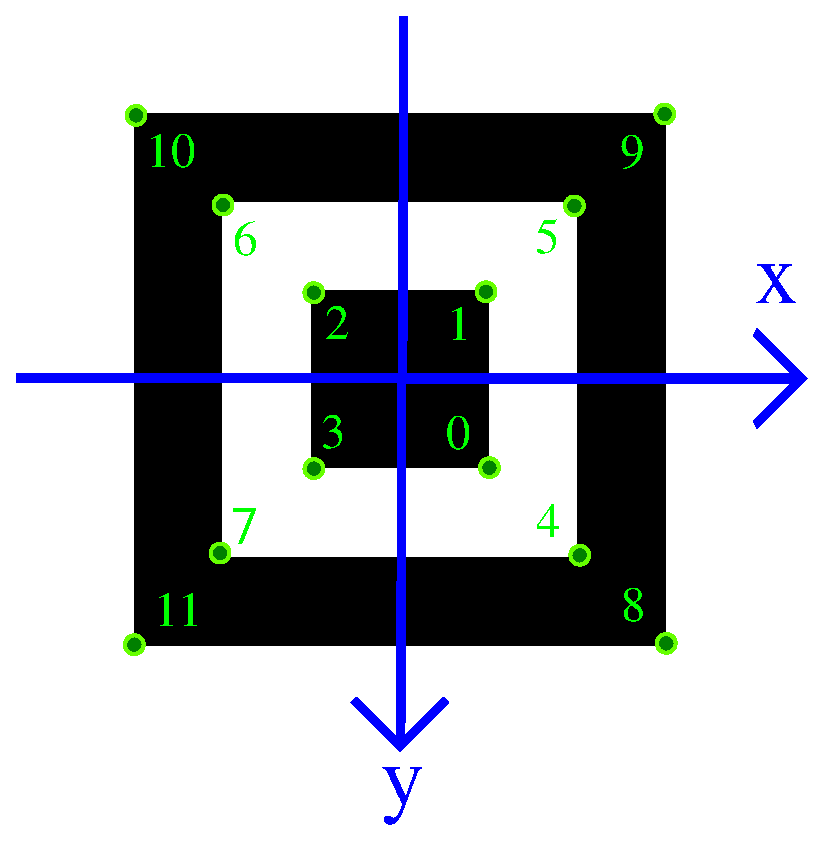
\includegraphics[scale=0.35]{figs_detection/QlSetDetail.eps}
\caption{Detalle de un $QlSet$. A la izquierda se muestra el resultado de la detecci�n de un $QlSet$ y el orden interno de sus cuadril�teros y a la derecha el orden de los v�rtices respecto al sistema de coordenadas local.}
\label{fig:QlSetDetail}
\end{figure}

Un detalle del marcador completo se muestra en la figura \ref{fig:MarkerDetail} en donde se define el conjunto $i$ de cuadril�teros conc�ntricos como el $QlSet[i]$ y se definen los respectivos centros de cada uno de ellos como $\mathbf{c}_i$. El sistema de coordenadas del marcador QR tiene centro en el centro del $QlSet[0]$ y ejes de coordenadas id�nticos al definido para cada $Ql$. Se tiene adem�s que los ejes de coordenadas pueden ser obtenidos mediante los vectores normalizados,
\begin{equation}
\begin{split}
\mathbf{x}  = \frac{\mathbf{c}_1 - \mathbf{c}_0}{||\mathbf{c}_1-\mathbf{c}_0||} & \quad
\mathbf{y}  = \frac{\mathbf{c}_2 - \mathbf{c}_0}{||\mathbf{c}_2-\mathbf{c}_0||}
\end{split} 
\label{ec:detection_ejes}
\end{equation}

La disposici�n de los $QlSet$ es tal que la distancia indicada $d_{01}$ definida como la norma del vector entre los centros $\mathbf{c}_1$ y $\mathbf{c}_0$ es significativamente mayor que la distancia $d_{02}$ definida como la norma del vector entre los centros $\mathbf{c}_2$ y $\mathbf{c}_1$. Esto es, $d_{01}\gg d_{02}$. Este criterio facilita la identificaci�n de los $QlSet$ entre s� basados �nicamente en la posici�n de sus centros y es explicado en la secci�n de determinaci�n de correspondencias (Secci�n \ref{sec:detection_correspondencias}).
\begin{figure}[h!]
\centering
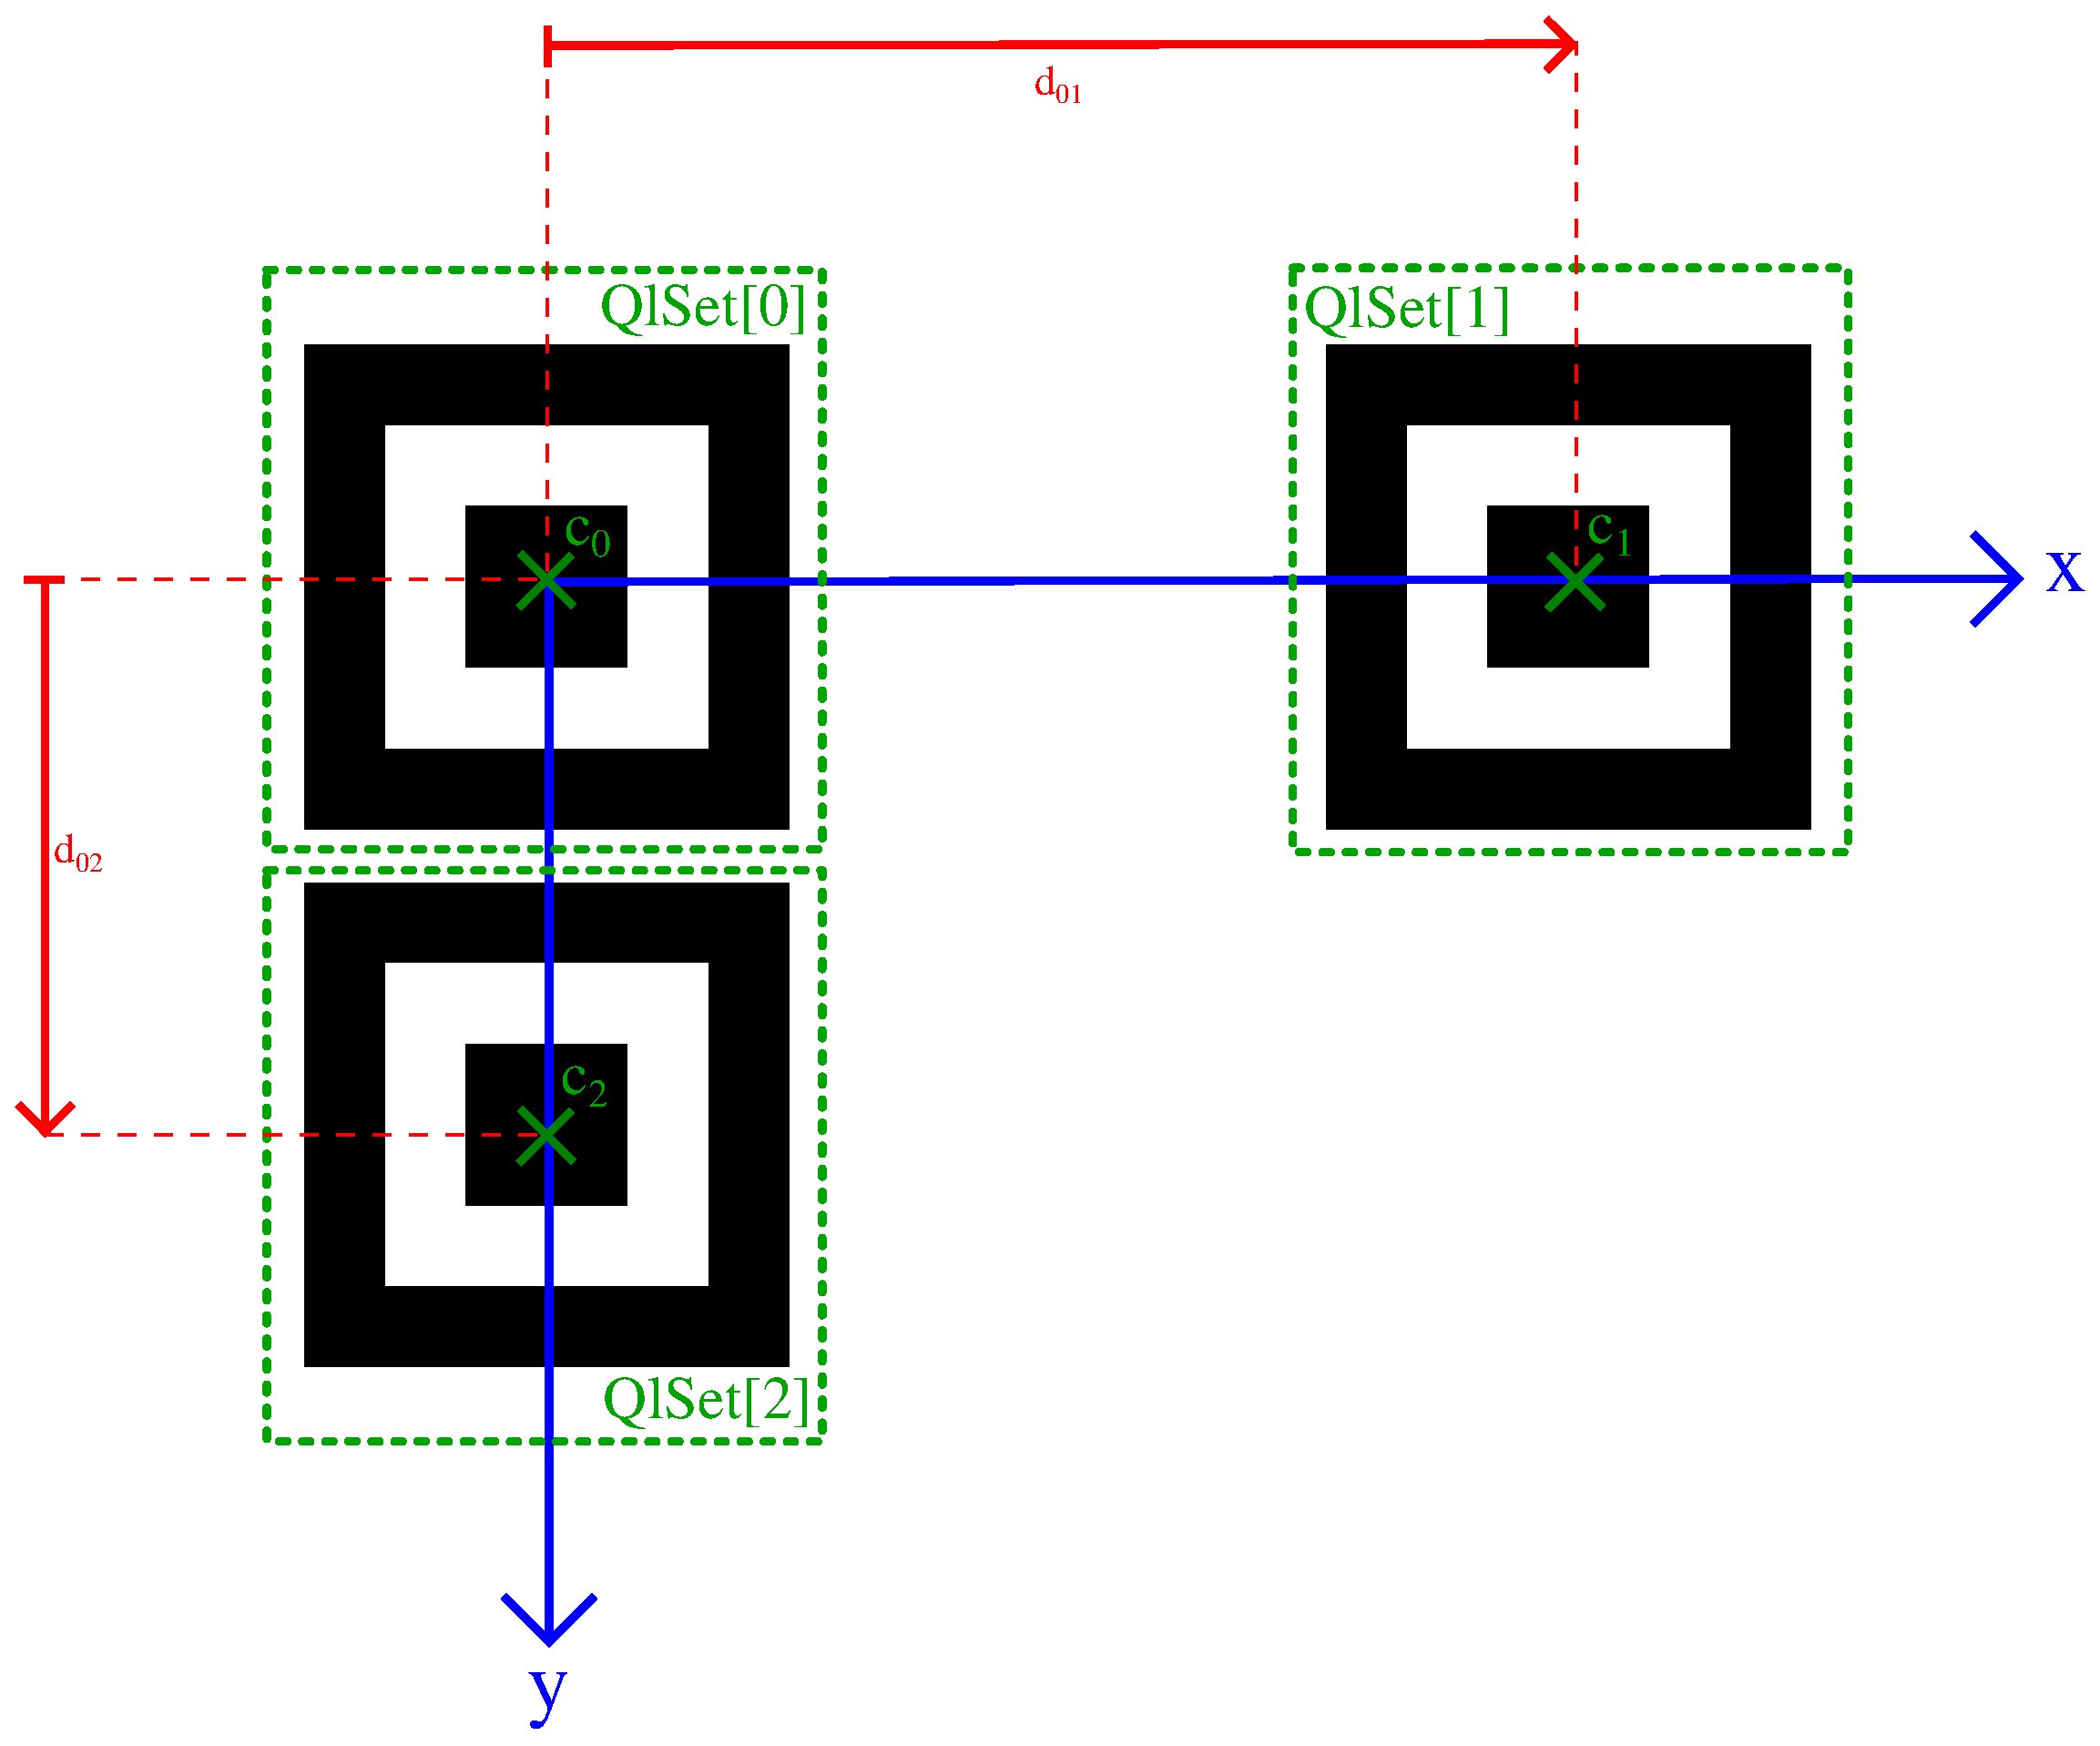
\includegraphics[scale=0.3]{figs_detection/MarkerDetail.eps}
\caption{Detalle del marcador propuesto formando un sistema de coordenadas.}
\label{fig:MarkerDetail}
\end{figure}


\subsection{Par�metros de dise�o}
Provisto el dise�o del marcador descrito, quedan definidos ciertos par�metros \textbf{estructurales} que fueron tomados fijos a lo largo del proyecto pero que podr�an ser cambiados para trabajos futuros asociados. Estos par�metros son:
\begin{itemize}
\item M: cantidad de conjuntos de cuadril�teros.
\item N: cantidad de cuadril�teros por conjuntos de cuadril�teros.
\item Geometr�a: geometr�a de los cuadril�teros ($Ql$).
\item Disposici�n: disposici�n espacial de los conjuntos de cuadril�teros ($QlSet$).
\end{itemize}

El criterio de elecci�n de $M$ y $N$ parte del dise�o los c�digos QR como ya fue explicado. La detecci�n por segmentos de l�nea resulta una cantidad de $3\times QlSet$'s conteniendo $3 \times Ql$'s cada uno. Bajo esta elecci�n de par�metros se tienen $36$ segmentos y v�rtices. Se tiene entonces un n�mero de puntos caracter�sticos razonable para la estimaci�n de pose.

La elecci�n de \emph{cuadrados} como par�metro de geometr�a se basa en la necesidad de tener igual resoluci�n en los dos ejes del marcador. De esta forma se asegura una distancia l�mite en donde, en un caso ideal enfrentado al marcador, la detecci�n de segmentos de l�nea falla simult�neamente en los segmentos verticales como en los horizontales. De otra forma se tendr�a una direcci�n que limita m�s que la otra desaprovechando resoluci�n.

La disposici�n espacial de los conjuntos de cuadril�teros esta en primer lugar limitada a un plano y en segundo lugar es tal que se puede definir ejes de coordenadas ortogonales mediante los centros como se muestra en la Figura \ref{fig:MarkerDetail}.\\

Por otro lado se tiene otro juego de par�metros \textbf{din�micos} que concluyen con el dise�o del marcador. Estos par�metros conservan la estructura intr�nseca del marcador permitiendo versatilidad en la aplicaci�n y sin la necesidad de modificaci�n alguna de los algoritmos desarrollados. Estos son:
\begin{itemize}
\item $d_{ij}$: distancia entre los centros $QlSet[j]$ con $QlSet[i]$.
\item $l$: lado del cuadril�tero m�s peque�o ($Ql[0]$) de los $QlSet$.
\end{itemize}

En este caso se debe cumplir siempre la condici�n impuesta previamente en donde $d_{01}\gg d_{02}$. De otra forma se deber�n realizar ciertas hip�tesis no gen�ricas o se deber� aumentar ligeramente la complejidad del algoritmo para la identificaci�n del marcador.\\

\subsection{Dise�o utilizado}
\textbf{Dise�o de Test}: Durante el desarrollo e implementaci�n de los algoritmos de detecci�n e identificaci�n de los v�rtices del marcador se trabaj� con determinados par�metros de dise�o de dimensiones apropiadas para posibilitar el traslado y las pruebas dom�sticas. 
\begin{itemize}
 \item $l = 30 mm$
 \item $d_{01} = 190 mm$
 \item $d_{02} = 100 mm$
\end{itemize}

\section{Detecci�n}
La etapa de detecci�n del marcador se puede separar en tres grandes bloques:
\begin{itemize}
 \item Detecci�n de segmentos de l�nea.
 \item Filtrado y agrupamiento de segmentos.
 \item Determinaci�n de correspondencias.
\end{itemize}
En esta secci�n se muestran algunos resultados para la detecci�n de segmentos de l�nea por LSD y se centra en profundidad en los algoritmos desarrollados durante el proyecto para el filtrado de segmentos y determinaci�n de correspondencias.

\subsection{Detecci�n de segmentos de l�nea}
La detecci�n de segmentos de l�nea se realiza mediante el uso del algoritmo LSD el cual se detalla en el Cap�tulo \ref{chap: lsd}. En forma resumida, dicho algoritmo toma como entrada una imagen en escala de grises de tama�o $W\times H$ y devuelve una lista de segmentos en forma de pares de puntos de origen y destino. 

En la Figura \ref{fig:resultado_lsd} se muestra un resultado para la detecci�n de segmentos de l�nea por LSD.
\begin{figure}[h!]
  \centering
  \subfigure[Entrada: imagen conteniendo al marcador]{
    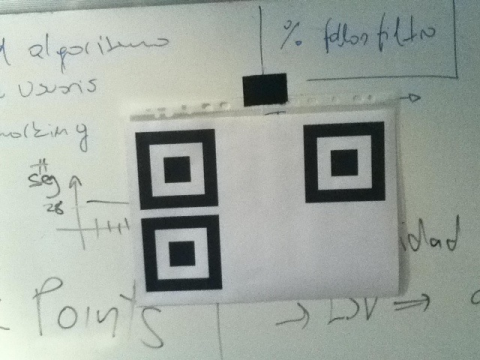
\includegraphics[scale=0.45]{figs_detection/img.png}}
  \subfigure[Salida: segmentos de l�nea detectados por LSD]{
    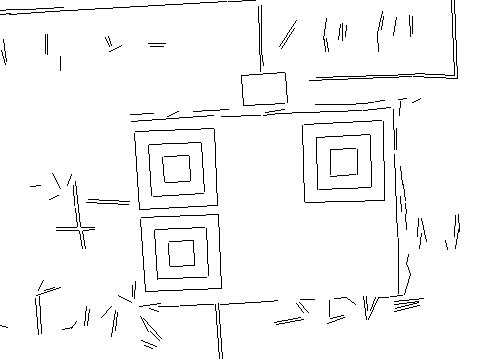
\includegraphics[scale=0.45]{figs_detection/lsd.png}}
  \caption{Resultados del algoritmo de detecci�n de segmentos de l�nea LSD.}
  \label{fig:resultado_lsd}
\end{figure}

\subsection{Filtrado y agrupamiento de segmentos}
El filtrado y agrupamiento de segmentos consiste en la b�squeda de conjuntos de cuatro segmentos conexos en la lista de segmentos de l�nea detectados por LSD. Los conjuntos de segmentos conexos encontrados se devuelven en una lista en el mismo formato a la de LSD pero agrupados de a cuatro. A continuaci�n se realiza una breve descripci�n del algoritmo de filtrado de segmentos implementado.\\

Se parte de una lista de $m$ segmentos de l�nea,
\begin{equation}
 \mathbf{L} = \begin{pmatrix}
               \mathbf{s}_0 & \mathbf{s}_1 & \dots & \mathbf{s}_{m-1} 
              \end{pmatrix}^t
\end{equation}
y se recorre en $i$ en busca de segmentos vecinos. La estrategia utilizada consiste en buscar, para el $i$-�simo segmento $\mathbf{s}_i$, dos segmentos vecinos. En una primera etapa $\mathbf{s}_j$ y en una segunda etapa $\mathbf{s}_k$, de forma que se forme una ``U'' como se muestra en la Figura \ref{fig:SegmentosRectas}. La tercer etapa de b�squeda consiste en completar ese conjunto con un cuarto segmento $\mathbf{s}_l$ que cierre la ``U''.

Dos segmentos $\mathbf{s}_i$ y $\mathbf{s}_j$ son vecinos si se cumple que la distancia eucl�dea entre puntos, $d_{ij}$, es menor a un cierto umbral para alguna de las combinaciones $\mathbf{p}_i\leftrightarrow \mathbf{p}_j$, $\mathbf{q}_i\leftrightarrow \mathbf{q}_j$, $\mathbf{p}_i\leftrightarrow \mathbf{q}_j$ o $\mathbf{q}_i\leftrightarrow \mathbf{p}_j$. En la primera etapa de la b�squeda se testean todas las posibilidades mientras que en la segunda etapa se testean solo los puntos del segmento que no fueron utilizados. Por ejemplo, si se encontr� la correspondencia $\mathbf{p}_i\leftrightarrow \mathbf{p}_j$ se busca el $k$-�simo segmento $\mathbf{s}_k$ que cumple que la distancia euclidiana $d_{ij}$ es menor a cierto umbral para alguna de las combinaciones $\mathbf{q}_i\leftrightarrow \mathbf{p}_k$ y $\mathbf{q}_i\leftrightarrow \mathbf{q}_k$. En la tercer etapa la chequeo se realiza de forma a�n m�s restringida probando para el segmento $\mathbf{s}_l$ correspondencia simult�nea entre sus puntos y solamente un punto cada uno de los segmentos $\mathbf{s}_j$ y $\mathbf{s}_k$ .\\
\begin{figure}[h!]
\centering
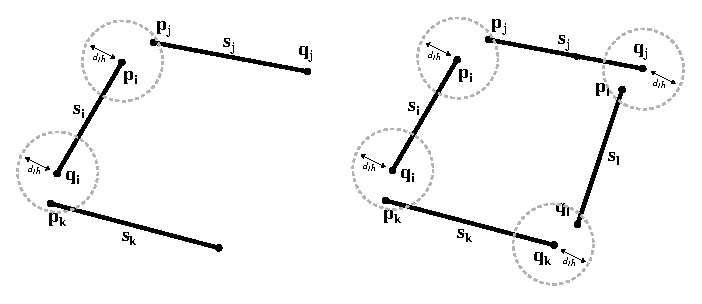
\includegraphics[scale=0.8]{figs_detection/SegmentosRectas.eps}
\caption{Conjunto de cuadril�teros conexos. A la izquierda la primera y segunda etapa del filtrado completadas para el segmento $\mathbf{s}_i$ en donde se busca una ``U''. A la derecha la �ltima etapa en donde se cierra la ``U'' con el segmento $\mathbf{s}_l$.}
\label{fig:SegmentosRectas}
\end{figure}

Una vez encontrado el conjunto de cuatro segmentos conexos estos se marcan como utilizados, se guardan en una lista de salida y se contin�a con el segmento $i+1$ hasta recorrer los $m$ segmentos de la lista de entrada. De esta forma se obtiene una lista de salida $\mathbf{S}$ de $n$ segmentos en donde $n$ es por construcci�n m�ltiplo de cuatro.\\

En la Figura \ref{fig:resultado_lsdfilt} se muestran lo resultados obtenidos para el algoritmo tomando como entrada la lista de segmentos de LSD. Se puede ver que los lados de los cuadrados del marcador son detectados correctamente pero tambi�n hay otras detecciones presentes. Por ejemplo el rect�ngulo negro correspondiente a un trozo de cinta negra que sostiene el marcador (ver Figura \ref{fig:resultado_lsd}(a)). Tambi�n sobreviven otro tipo de elementos indeseados que se explican a continuaci�n.
\begin{figure}[h!]
  \centering
  \subfigure[Entrada: segmentos de l�nea detectados por LSD]{
    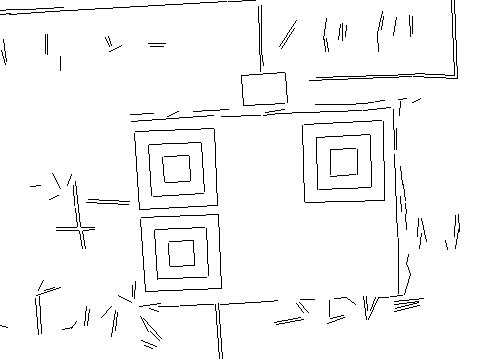
\includegraphics[scale=0.45]{figs_detection/lsd.png}}
  \subfigure[Salida: segmentos de l�nea filtrados y agrupados]{
    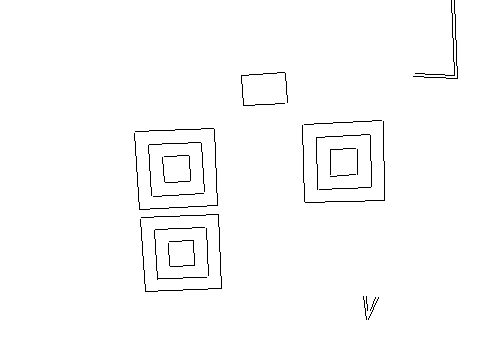
\includegraphics[scale=0.45]{figs_detection/lsdfilt.png}}
  \caption{Resultados del algoritmo de filtrado y agrupamiento de segmentos de l�nea.}
  \label{fig:resultado_lsdfilt}
\end{figure}

El algoritmo descrito es simple y provee resultados aceptables en general pero es propenso a tanto a detectar \emph{falsos positivos} como al \emph{sobre-filtrado} algunos conjuntos. 

La detecci�n de falsos positivos se puede atribuir principalmente a la condici�n de vecindad utilizada en donde un caso como el que se muestra en la Figura \ref{fig:FilterError} de un conjunto de segmentos paralelos cercanos y de tama�o similar ``sobrevive'' al filtrado de segmentos. De forma de evitar estos  falsos positivos, se podr�a considerar implementar un condici�n de vecindad que tome en cuenta el punto de  intersecci�n entre los segmentos y la distancia de este punto a los puntos $\mathbf{p}$, $\mathbf{q}$ m�s cercanos de cada segmento. Como se explicar� en le Secci�n \ref{sec:detection_correspondencias}, debido a que el algoritmo de determinaci�n de correspondencias realiza la intersecci�n entre estos segmentos se puede chequear alguna condici�n sobre los segmentos o su intersecci�n y en ese momento filtrar estos casos.
\begin{figure}[h!]
\centering
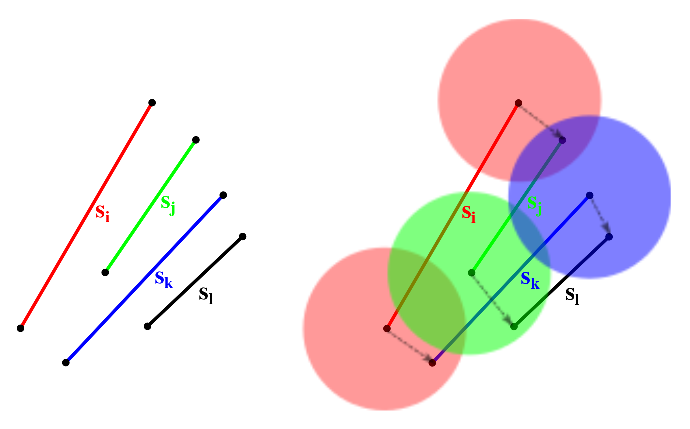
\includegraphics[scale=0.8]{figs_detection/FilterError.eps}
\caption{Posible configuraci�n de segmentos paralelos que ``sobreviven'' al filtrado. A la izquierda el grupo de segmentos, a la derecha se muestra como se desarrolla el filtrado de $\mathbf{s}_i$.}
\label{fig:FilterError}
\end{figure}

El sobre-filtrado de segmentos tiende a ocurrir cuando no se cumple la condici�n de distancia entre segmentos vecinos cuando visualmente si lo son. Se debe principalmente a que se utiliza para el filtrado un valor de $d_{th}$ fijo que conduce a buenos resultados para la aplicaci�n pero en ciertas circunstancias produce este problema. Esta medida de distancia se podr�a tomar relativa al largo del los segmentos a \emph{testear} de forma de generalizar el valor pero se deber�a analizar un poco m�s en detalle la posible implementaci�n para que resulte en buenos resultados y no introduzca otra clase de errores.\\

El algoritmo de filtrado y agrupamiento de segmentos es sensible respecto a la elecci�n del par�metro $d_{th}$. Si este par�metro est� por debajo del valor �ptimo la \emph{performance} del algoritmo se ver� afectada fuertemente, pues se corre el riesgo de sobre filtrar y no proporcionar suficientes segmentos para la correcta determinaci�n de correspondencias. Por el contrario, si el par�metro est� por encima del valor �ptimo, el filtrado tiende a proveer falsos positivos, aunque este caso no llega a ser tan cr�tico como el primero para la aplicaci�n. A modo de ejemplo, para una imagen de tama�o $480 \times 320$ con el marcador ocupando entre un $25\%$ y un $80\% $ el valor del par�metro que da mejores resultados es aproximadamente de $6$ o $7$ p�xeles.

\subsection{Determinaci�n de correspondencias}
\label{sec:detection_correspondencias}
Se detalla a continuaci�n el algoritmo de determinaci�n de correspondencias a partir de grupos de cuatro segmentos de l�nea conexos. Para ese algoritmo se hace uso de los elementos estructurales del marcador vistos en la Secci�n \ref{sec:detection_estructuras}, de forma de desarrollar un algoritmo modular, escalable y simple.

Se toma como entrada la lista de segmentos filtrados y agrupados
\begin{equation}
\mathbf{S} = \begin{pmatrix}
			 \mathbf{s}_0 & \mathbf{s}_1 & \dots & \mathbf{s}_{i} & \mathbf{s}_{i+1} & \mathbf{s}_{i+2} & \mathbf{s}_{i+3} & \dots & \mathbf{s}_{n-1}
			 \end{pmatrix}^t
\end{equation}
en donde cada segmento se compone de un punto inicial $\mathbf{p}_{i}$ y un punto final $\mathbf{q}_{i}$, $\mathbf{s}_{i} = (\mathbf{p}_{i},\mathbf{q}_{i})$, con $n$ m�ltiplo de cuatro. Si $i$ tambi�n lo es, entonces el sub-conjunto, 
$\mathbf{S}_i = \begin{pmatrix}
				\mathbf{s}_{i} & \mathbf{s}_{i+1} & \mathbf{s}_{i+2} & \mathbf{s}_{i+3}
				\end{pmatrix}^t$, corresponde a un conjunto de cuatro segmentos del l�nea conexos.

Para cada sub-conjunto $\mathbf{S}_i$ se intersectan entre s� los segmentos obteniendo una lista de cuatro v�rtices,
$\mathbf{V}_i =  \begin{pmatrix}
		 \mathbf{v}_{i} & \mathbf{v}_{i+1} & \mathbf{v}_{i+2} & \mathbf{v}_{i+3} 
		 \end{pmatrix}^t$. 
Si  $\mathbf{r}_i$ es la recta que pasa por los puntos $\mathbf{p}_i$ y $\mathbf{q}_i$ del segmento  $\mathbf{s}_i$, la lista de v�rtices se obtiene como sigue,
\begin{eqnarray}
\mathbf{v}_i = & \mathbf{r}_i\cap \mathbf{r}_{i+1} \nonumber\\
\mathbf{v}_{i+1} = & \mathbf{r}_i\cap \mathbf{r}_{i+2} \nonumber\\
\mathbf{v}_{i+2} = & \mathbf{r}_{i+3}\cap \mathbf{r}_{i+2} \nonumber\\
\mathbf{v}_{i+3} = & \mathbf{r}_{i+3}\cap \mathbf{r}_{i+1} \nonumber
\end{eqnarray}
resultando en dos posibles configuraciones de v�rtices. Las dos configuraciones se muestran en la Figura \ref{fig:Vertices} en donde una de ellas tiene sentido horario y la otra antihorario partiendo de ${v}_i$.
\begin{figure}[h!]
\centering
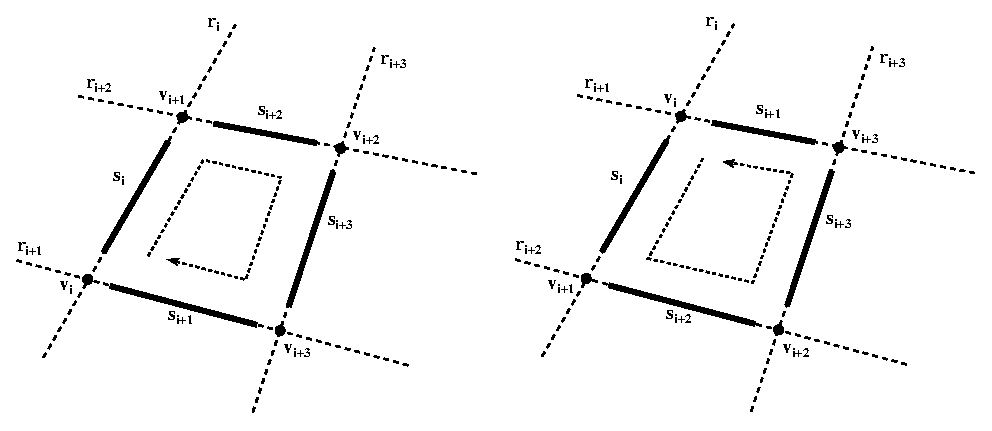
\includegraphics[scale=0.8]{figs_detection/Vertices.eps}
\caption{Posibles configuraciones de v�rtices posterior a la intersecci�n de conjuntos de segmentos pertenecientes a un cuadril�tero.}
\label{fig:Vertices}
\end{figure}

Posterior a la intersecci�n se realiza un chequeo sobre el valor de las coordenadas de los v�rtices. Si alguno de ellos se encuentra fuera de los l�mites de la imagen, el conjunto de cuatro segmentos es marcado como inv�lido. Este chequeo resulta en el filtrado de ``falsos cuadril�teros'' corrigiendo un defecto del filtrado de segmentos, como por ejemplo un grupo de segmentos paralelos cercanos como ya se explic�. 

Para cada uno de los conjuntos de v�rtices se construye con ellos un elemento cuadril�tero que se almacena en una lista de cuadril�teros
\begin{eqnarray*}
 QlList =  \begin{pmatrix}
            Ql[0] & Ql[1] & \dots & Ql[i] & \dots & Ql[\frac{n}{4}]
           \end{pmatrix}^t
\end{eqnarray*}
% en sentido amplio, de dos segmentos contiguos, $s_i\cap s_{i+1}$ dadas las recta $r_1$ que pasa por los puntos $\mathbf{p}_1$, $\mathbf{q}_1$ del segmento $s_1$ y la recta $r_2$ que pasa por los puntos $\mathbf{p}_2$, $\mathbf{q}_2$ del segmento $s_2$, se determina el v�rtice correspondiente como la intersecci�n $r_1 \cap r_2$. \\
% 
% y se intersectan en grupos de cuatro obteniendo cuatro v�rtices por cada grupo. Para cada grupo de v�rtices $v_k$ se construye un elemento cuadril�tero $\text{Ql}[k]$ que se almacena en una lista de cuadril�teros. 

A partir de esa lista de cuadril�teros, se buscan grupos de tres cuadril�teros $QlSet$ que ``compartan'' un mismo centro. Para esto se recorre ordenadamente la lista en $i$ buscando para cada cuadril�tero dos cuadril�teros $j$ y $k$ que cumplan que la distancia entre sus centros  y el del $i$-�simo cuadril�tero sea menor a cierto umbral $c_{th}$,
\begin{equation}
\begin{split}
 d_{ij} = ||\mathbf{c}_i - \mathbf{c}_j||<c_{th}, & \quad  d_{ik} = ||\mathbf{c}_i - \mathbf{c}_k||<c_{th}.
\end{split}
\end{equation}
Estos cuadril�teros se marcan en la lista como utilizados con ellos se forma el $l$-�simo $QlSet$ orden�ndolos seg�n su per�metro, de menor a mayor como  
$$QlSet[l] = \begin{pmatrix} Ql[0] & Ql[1] & Ql[2] \end{pmatrix}$$
con $l = (0,1,2)$. Esta b�squeda se realiza hasta encontrar un total de tres $QlSet$ completos de forma de obtener un marcador completo, esto es, detectando todos los cuadril�teros que lo componen. \\

Una vez obtenida la lista de tres $QlSet$, 
$$QlSetList = \begin{pmatrix} QlSet[0] & QlSet[1] & QlSet[2] \end{pmatrix}$$
�sta se ordena de forma que su disposici�n espacial se corresponda con la del marcador QR. Para esto se calculan las distancias entre los centros de cada $QlSet$ y se toma el �ndice $i$ como el �ndice que produce el vector de menor distancia, $\mathbf{u}_i = \mathbf{c}_{i+1} -\mathbf{c}_i$. En este punto es importante que la condici�n de distancia entre los centros de los $QlSet$ se cumpla, $d_{10} \gg d_{20}$, para una simple identificaci�n. Bajo una transformaci�n proyectiva del marcador, es posible que esta relaci�n se modifique e incluso que deje de valer, pero imponiendo la condici�n ``mucho mayor'' se asegura que el algoritmo funciona correctamente para condiciones razonables. Esto es, para proyecciones o poses que se encuentran dentro de las hip�tesis de uso de la aplicaci�n.

Una vez seleccionado el vector $\mathbf{u}_i$, se tienen obtiene el juego de vectores $(\mathbf{u}_i,\mathbf{u}_{i+1},\mathbf{u}_{i+2})$ como se muestra en la figura \ref{fig:Centros}.
\begin{figure}[h!]
\centering
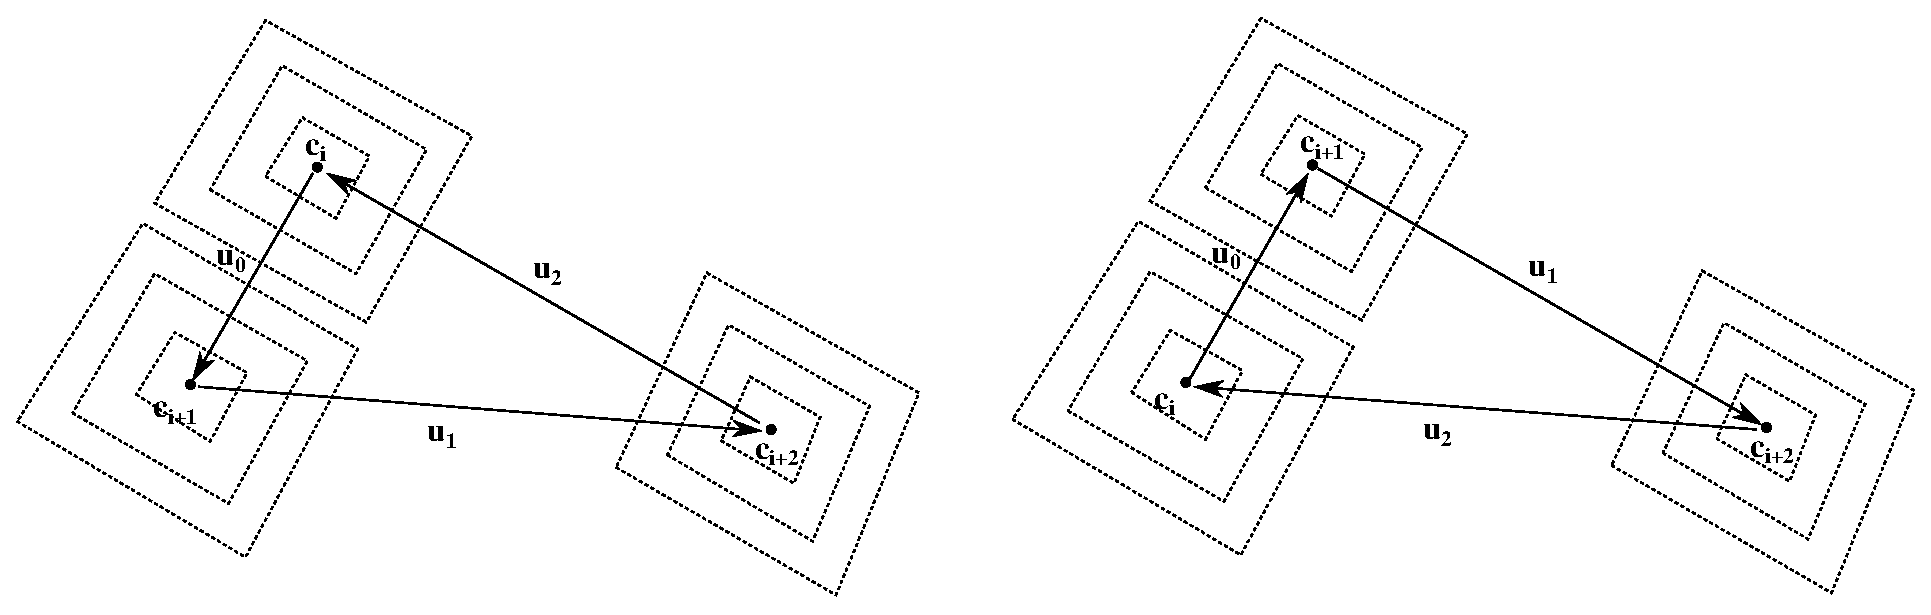
\includegraphics[scale=0.45]{figs_detection/Centros.eps}
\caption{V�rtices de cada $Ql$ ordenados respecto al signo de sus proyecciones contra el sistema de coordenadas local a cada $QlSet$.}
\label{fig:Centros}
\end{figure}

Existen solo dos posibles configuraciones para estos vectores por lo que se utiliza este conocimiento para ordenar los $QlSet$ de la lista realizando el producto vectorial, aumentando la dimensi�n de los vectores $\hat{\mathbf{u}_i}$ y $\hat{\mathbf{u}_{i+1}}$ con coordenada $z=0$,
\begin{equation*}
 \mathbf{b} = \hat{\mathbf{u}_i} \times \hat{\mathbf{u}_{i+1}}.
\end{equation*}
Si el vector $\mathbf{b}$ tiene valor en la coordenada $z$ positivo se ordena como,
\begin{eqnarray*}
 QlSet[0]\longleftarrow & QlSet[i]\\
 QlSet[1]\longleftarrow & QlSet[i+2]\\
 QlSet[2]\longleftarrow & QlSet[i+1]
\end{eqnarray*}
o de lo contrario se ordena como,
\begin{eqnarray*}
 QlSet[0]\longleftarrow & QlSet[i+1]\\
 QlSet[1]\longleftarrow & QlSet[i+2]\\
 QlSet[2]\longleftarrow & QlSet[i]
\end{eqnarray*}

Por ultimo se construye un marcador QR que contiene la lista de tres $QlSet$ ordenados seg�n lo indicado permitiendo la definici�n de un centro de coordenadas como el centro $\mathbf{c}_0$ del $QlSet[0]$ y ejes de coordenadas definidos en la Ecuaci�n \ref{ec:detection_ejes}. Los ejes de este sistema de coordenadas permiten, para cada $Ql$ de cada $QlSet$, proyectar los v�rtices sobre el sistema de coordenadas local al $QlSet$ y seg�n su signo ordenarlos como se muestra en la Figura \ref{fig:VerticesProyectados}.
\begin{figure}[h!]
\centering
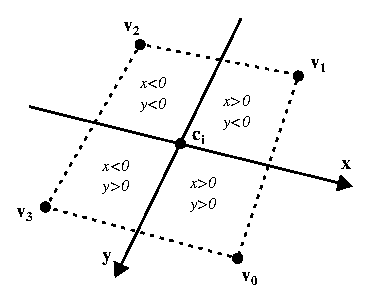
\includegraphics[scale=0.8]{figs_detection/VerticesProyectados.eps}
\caption{Posibles configuraciones de centros resultan en la orientaci�n de los vectores $\mathbf{u}_{i+k}$.}
\label{fig:VerticesProyectados}
\end{figure}
De esta forma, recorriendo ordenadamente los elementos del marcador, se ordenan los v�rtices de cada $Ql$ del marcador.\\

Por �ltimo, a partir del marcador ordenado, se extrae una lista de v�rtices que se corresponde con la lista de v�rtices del marcador en coordenadas del mundo. Este recorrido se realiza en el siguiente orden,
\begin{algorithm}
\For{$i=(0,1,2)$}
  { \For{$j=(0,1,2)$}
  { \For{$k=(0,1,2,3)$} {
    So obtiene el punto v�rtice: $\mathbf{p} = QlSet[i] \rightarrow Ql[j] \rightarrow v[k]$\;
    Se agrega a la lista de correspondencias $\mathbf{m}_{l} \leftarrow \mathbf{p}$\;
    Se incrementa $l$;
  }}}
\end{algorithm}

Se determinan las correspondencias $\mathbf{M}_i\leftrightarrow \mathbf{m}_i$ necesarias para la estimaci�n de pose las cuales se muestran en la Figura \ref{fig:resultado_points}. Se puede ver que el algoritmo de determinaci�n de correspondencias funciona correctamente por lo que los ``falsos'' cuadril�teros que sobreviven al filtrado de segmentos no son un problema.
\begin{figure}[h!]
  \centering
  \subfigure[Entrada: segmentos de l�nea filtrados y agrupados]{
    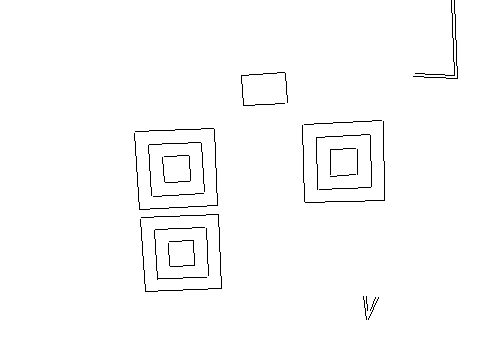
\includegraphics[scale=0.45]{figs_detection/lsdfilt.png}}
  \subfigure[Salida: puntos v�rtices ordenados.]{
    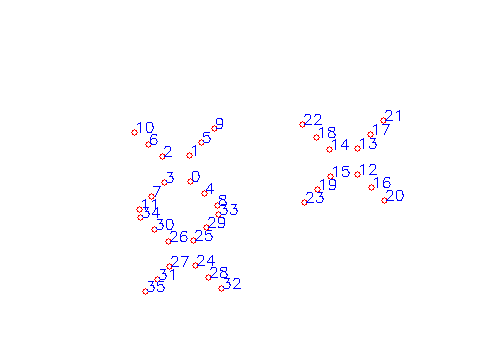
\includegraphics[scale=0.45]{figs_detection/points.png}}
  \caption{Resultados del algoritmo de determinaci�n de correspondencias.}
  \label{fig:resultado_points}
\end{figure}

\subsection{Detecci�n robusta}
El algoritmo descripto al momento requiere que dentro de la lista de segmentos filtrados se encuentren todos los segmentos que componen el marcador pero este requerimiento representa un problema importante en cuanto a el desempe�o del algoritmo. En caso de que esto no se cumpla no es posible proporcionar las correspondencias necesarias para la estimaci�n de pose y no se tendr� una pose v�lida para ese cuadro o \emph{frame} para la aplicaci�n. En aplicaciones en tiempo real en donde el procesamiento de la imagen es la mayor limitante, la fluidez visual dada por el \emph{frame rate} se ve notablemente perjudicada resultando en que el sistema sea inc�modo e incluso inutilizable. Es por esto que en esta secci�n se desarrolla la extensi�n del algoritmo de determinaci�n de correspondencias para una cantidad menor de segmentos detectados y filtrados que resulta en una mejora sustancial en la cantidad de \emph{frames} en los cuales es posible determinar correspondencias y obtener as� una pose v�lida.

Se busca una determinaci�n de correspondencias m�s robusta pero manteniendo las esencia del algoritmo desarrollado. Por esto se tienen dos aspectos a tomar en cuenta; la detecci�n de $QlSet$'s se realiza basada en la b�squeda de cuadril�teros conc�ntricos por lo que se debe contar con un m�nimo de dos cuadril�teros por $QlSet$ para permitir la diferenciaci�n entre un conjunto de segmentos filtrados debido a que pertenecen al marcador y a otro conjunto que no pertenece pero si cumple con las condiciones, por ejemplo podr�a ser el marco de una obra o cualquier elemento en la escena que forme un cuadril�tero. Esto fija un l�mite de no menos de $24$ segmentos necesarios para el funcionamiento. El otro aspecto a tomar en cuenta se refiere a la forma en que se ordenan los $Ql$'s dentro de cada $QlSet$. Como ya se explic� el orden se basa en la medida del per�metro de los $Ql$'s ordenando de menor a mayor por lo que ser� necesario contar con, al menos, un $QlSet$ completo de forma de tener una referencia a la hora de identificar los $QlSet$'s incompletos hallados. Por lo tanto la extensi�n del algoritmo permite una correcta identificaci�n de los v�rtices del marcador con un n�mero mayor o igual a $28$ segmentos.\\

La implementaci�n de esta extensi�n del algoritmo se realiz� manteniendo la estructura b�sica descrita anteriormente y se detalla aqu� solamente los agregados realizados.

Al realizar la b�squeda de conjuntos de cuadril�teros conc�ntricos se buscan en primer lugar los $QlSet$'s completos y luego en caso de que estos no lleguen a ser tres, se intenta completar buscando $QlSet$'s incompletos o sea conjuntos de dos cuadril�teros que comparten un mismo centro. Estos se agrupan en una lista de la misma forma en que se describi� anteriormente pero dejando el tercer cuadril�tero, $Ql[2]$, marcado como inv�lido.

Una vez completada la lista de tres $QlSet$, con al menos uno de ellos detectado completo, se ordenan en primer lugar los $QlSet$ completos y de ellos se extrae una lista de per�metros promedio. Esta lista de per�metros promedio se utiliza para el ordenamiento de los $QlSet$ incompletos comparando con los per�metros de los $Ql[0]$ y $Ql[1]$ de cada $QlSet$. El $Ql[2]$ previamente marcado como inv�lido se posiciona por descarte en la posici�n que corresponda.

Al momento de proporcionar la lista de v�rtices ordenados $\mathbf{m}_i$ y correspondientes con los del modelo $\mathbf{M}_i$, se introducen valores inv�lidos para los $Ql$'s marcados como inv�lidos. Por �ltimo se realiza un recorte de las dos listas de puntos en base a estos valores inv�lidos, se recorre la lista de puntos en la imagen $\mathbf{m}_i$ y se extraen de la lista de puntos en la imagen y de los puntos del modelo los puntos inv�lidos obteniendo un juego de al menos $28$ correspondencias $\mathbf{m}_i' \leftrightarrow \mathbf{M}'_i$ para el algoritmo de estimaci�n de pose.\\

En la Figura \ref{fig:resultado_inc_points}(a) se muestran imagen en la que falla el filtrado de segmentos para uno de los cuadril�teros mientras que en la figura \ref{fig:resultado_inc_points}(b) se puede ver como el algoritmo de determinaci�n de correspondencias provee $32$ correspondencias ordenadas correctamente, diferenciando en el $QlSet$ incompleto los v�rtices.
\begin{figure}[h!]
  \centering
  \subfigure[Entrada: segmentos de l�nea filtrados y agrupados]{
    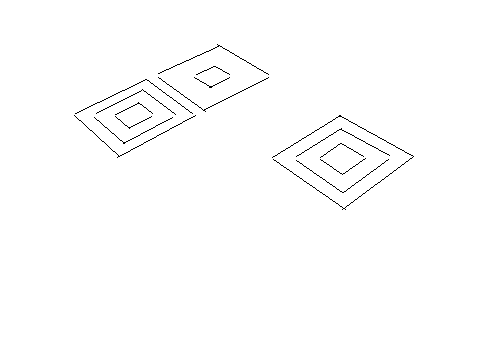
\includegraphics[scale=0.45]{figs_detection/mrkr_incompleto/lsdfilt.png}}
  \subfigure[Salida: puntos v�rtices ordenados.]{
    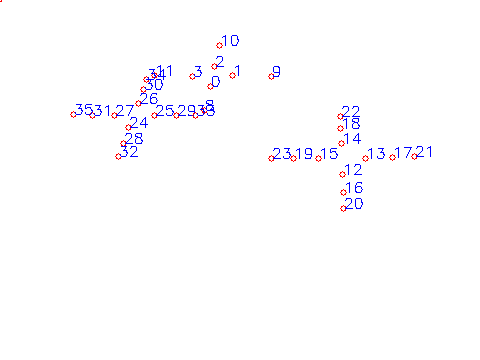
\includegraphics[scale=0.45]{figs_detection/mrkr_incompleto/points.png}}
  \caption{Resultados del algoritmo de determinaci�n de correspondencias robusto para una falla en el filtrado de segmentos.}
  \label{fig:resultado_inc_points}
\end{figure}

% La detecci�n de segmentos puede fallar debido a que las dimensiones del marcador en el plano de imagen sean peque�as y que la detecci�n de segmentos deje de ser estable. Tambi�n debido a oclusiones o ``segmentos'' partidos. Por otro lado debido a la simplicidad del algoritmo de filtrado y agrupamiento de segmentos, en particular debido simplicidad de la condici�n de vecindad, el algoritmo es propopenso a fallas por ejemplo filtrando un conjunto de cuatro segmentos cuando en la detecci�n de segmentos se puede ver que estan all�. puede fallar.

\section{Comentarios sobre la implementaci�n de los algoritmos}
Los algoritmos desarrollados en el presente cap�tulo fueron implementados en Lenguaje C y est�n autocontenidos en el mismo c�digo fuente sin la utilizaci�n de librer�as externas para su funcionamiento.\\

La elecci�n del lenguaje y la filosof�a de desarrollo comentada atr�s permite \textbf{portabilidad} en el uso de los mismos para aplicaciones m�s all� del proyecto y es un ejercicio de aprendizaje necesario. El algoritmo de filtrado y agrupamiento se implement� en los archivos \texttt{segments.c} y \texttt{segments.h} mientras que el de determinaci�n de correspondencias se implement� en los archivos \texttt{marker.c} y \texttt{marker.h}.\\

El entorno de desarrollo (IDE) utilizado para la implementaci�n fue Eclipse CDT para C/C++: \url{http://www.eclipse.org/cdt/} en un proyecto que utiliza un \emph{Makefile} para la compilaci�n por lo que se podr�a utilizar otro entorno en caso de ser necesario.\\

Adicionalmente de forma de facilitar la tareas de interfaz como el abrir/capturar, el guardado/despliegue de im�genes o video as� como el dibujado de segmentos y puntos sobre las im�genes se utiliza la librer�a OpenCV. Se aclara que esta interfaz no est� de ninguna forma integrada con los algoritmos desarrollados pero fue de gran utilidad para la implementaci�n de los mismos. Su utilizaci�n esta intr�nsecamente ligada a la librer�a OpenCV pero esta es una muy popular librer�a multifplataforma para procesamiento de im�genes.

\section{Resultados de Benchmark}
En esta secci�n se presentan algunos resultados de \emph{Benchmark} para los algoritmos de asociados a la detecci�n del marcador dise�ado. En particular se estudian los l�mites para la detecci�n de segmentos mediante LSD y el filtrado y agrupamiento de los mismos para juegos de im�genes sint�ticas generadas utilizando las herramientas explicadas en el Cap�tulo \ref{chap: benchmark}.\\

Se analizan los casos que presentaron limitaciones m�s significativas como, la profundidad m�xima del marcador respecto al eje $z$, la rotaci�n m�xima permitida sobre el eje $x$ y lo mismo para la rotaci�n sobre el eje $y$. Mediante este an�lisis se obtienen cotas \emph{pseudo-te�ricas} para establecer las limitaciones pr�cticas de uso de los algoritmos.\\

\subsection{Elecci�n de par�metros para Benchamark}
Para la evaluaci�n de los algoritmos se utilizaron algunos par�metros de Benchmark fijos y otros modificables llevando a una elecci�n definitiva de par�metros.\\

Un juego de par�metros fue tomado fijo y se refiere a la c�mara utilizada. 
\begin{itemize}
 \item $width \times height$: Tama�o de imagen tomado $480\times360$.
 \item $fov$: Campo visual referido al ancho tomado $46.46�$
 \item $centro$: Centro de la c�mara siempre ubicado en el medio de la imagen.
\end{itemize}

A lo largo de las diferentes pruebas realizadas se probaron modificar algunos par�metros para ver como estos afectaban los resultados. Los par�metros modificables son:
\begin{itemize}
 \item $d_{th}$: Distancia del threshold de filtrado de segmentos.
 \item $s$: Escala del LSD.
 \item $width \times height$: Tama�o de imagen.
\end{itemize}
Los valores que toman estos par�metros para las pruebas finales que corresponden con las que se muestran:
\begin{itemize}
 \item $d_{th} = 5px$
 \item $s = 0.5$
 \item $width\times height = 480\times360 px$
\end{itemize}
La elecci�n de estos par�metros fue \textbf{definitiva} para las pruebas de Benchmark a lo largo de todo el documento. Por m�s informaci�n sobre las herramientas de Benchmark y los par�metros ajustables para la generaci�n de im�genes sint�ticas referirse al Cap�tulo \ref{chap: benchmark}.

\newpage
\subsection{L�mite en profundidad: Eje z}
Para realizar las pruebas del l�mite de profundidad del marcador se gener� un juego de im�genes (\emph{Caso 1}) en las cuales el marcador se ubica enfrentado a la c�mara con el centro del mismo coincidente con el centro �ptico de la c�mara y por lo tanto en el centro de la imagen. Se utilizan profundidades que var�an desde $z=600mm$ hasta $z=2100mm$ de a $1mm$. \\

Se puede ver en la Figura \ref{fig:benchmark_segmentos_z} los casos l�mite sobre el cual el LSD no provee resultados satisfactorios y tambi�n el caso l�mite inmediatamente anterior a la falla del filtrado de segmentos. Se puede concluir que para el caso de profundidad el detector de segmentos LSD limita primero a una distancia de $z=1575mm$.
\begin{figure}[H]
  \centering
  \subfigure[Resultado de LSD para $z= 1575 mm$]{
    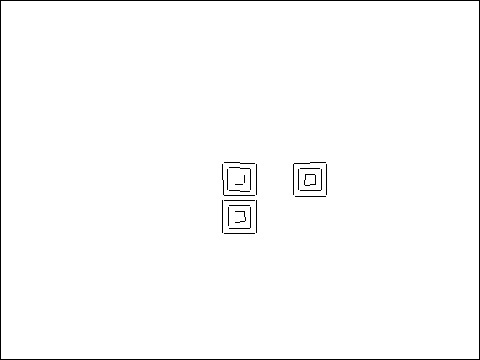
\includegraphics[scale=0.48]{figs_detection/limitesDeteccion/Caso1-LSD196.png}}
  \subfigure[Resultado de LSD para $z= 1580 mm$]{
    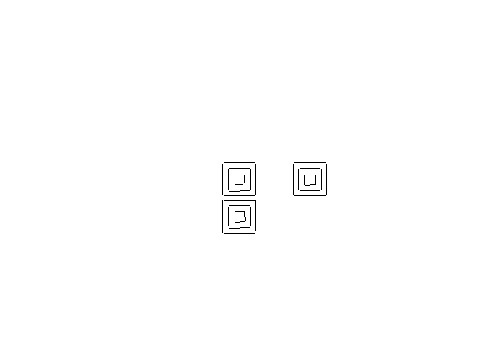
\includegraphics[scale=0.48]{figs_detection/limitesDeteccion/Caso1-LSD197.png}}
  \subfigure[Resultado de filtrado de segmentos para $z= 1575 mm$]{
    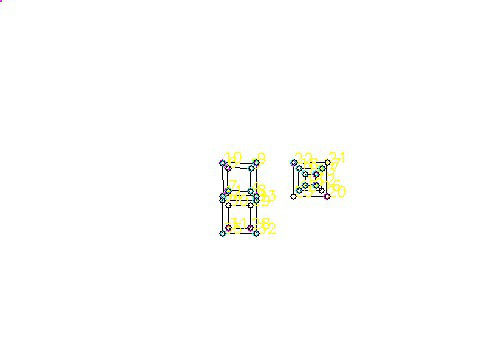
\includegraphics[scale=0.48]{figs_detection/limitesDeteccion/Caso1-LSDfilter196.png}}
  \caption{L�mites para la profundidad m�xima en el eje $z$ del marcador.}
  \label{fig:benchmark_segmentos_z}
\end{figure}

\newpage
\subsection{L�mite en rotaci�n: Eje x}
Para las pruebas del l�mite de rotaci�n sobre el eje $x$ del marcador se gener� un juego de im�genes (\emph{Caso 3}) en las cuales el marcador se ubica a una distancia fija de $z=1000mm$ con el centro del mismo coincidente con el centro �ptico de la c�mara y por lo tanto en el centro de la imagen. Sobre esta traslaci�n se varia la rotaci�n en el eje $x$ de a $2�$ desde $r_x = -60�$ hasta $r_x = 60�$.\\

Se puede ver en las Figuras \ref{fig:benchmark_segmentos_rx}(a) y \ref{fig:benchmark_segmentos_rx}(b) los casos de l�mite negativos y positivos respectivamente en los cuales el LSD falla. Debido a la asimetr�a del marcador limitan primero las rotaciones negativas. Por otro lado en las Figuras \ref{fig:benchmark_segmentos_rx}(c) y  \ref{fig:benchmark_segmentos_rx}(d) se observan los casos de l�mite negativos y positivos respectivamente inmediatamente anteriores a la falla del filtrado de segmentos. Se puede concluir que para las rotaciones sobe el eje $x$ limita LSD ya que el filtrado de segmentos funciona correctamente para casos inmediatamente anteriores.
\begin{figure}[H]
  \centering
  \subfigure[Resultado de LSD para $r_x= -52 �$]{
    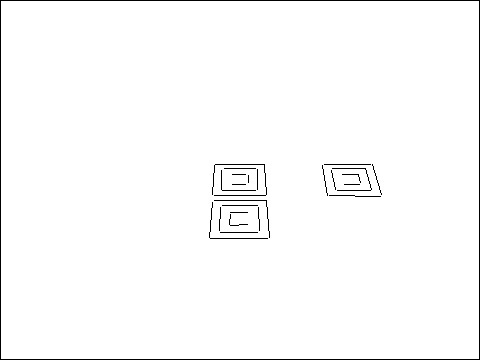
\includegraphics[scale=0.48]{figs_detection/limitesDeteccion/Caso3-LSD5.png}}
  \subfigure[Resultado de LSD para $r_x= 56 �$]{
    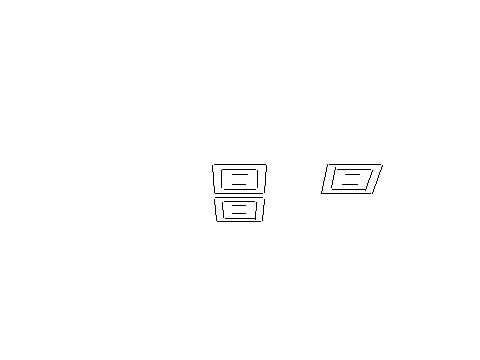
\includegraphics[scale=0.48]{figs_detection/limitesDeteccion/Caso3-LSD59.png}}
  \subfigure[Resultado de filtrado de segmentos para $r_x= -50 �$]{
    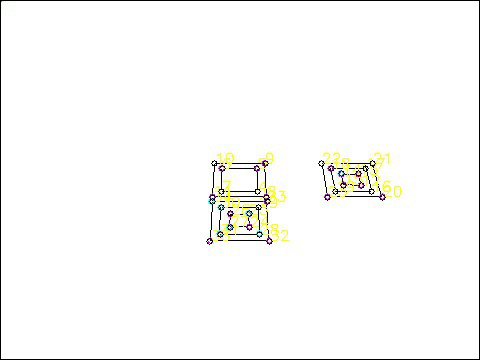
\includegraphics[scale=0.48]{figs_detection/limitesDeteccion/Caso3-LSDfilter6.png}}
  \subfigure[Resultado de filtrado de segmentos para $r_x= 54 �$]{
    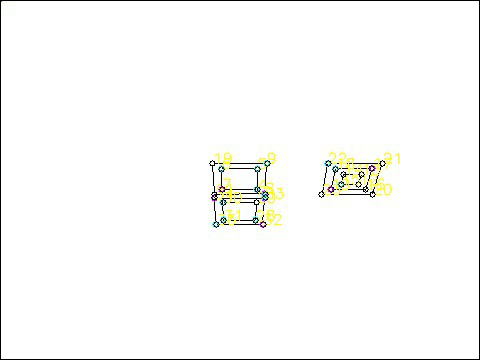
\includegraphics[scale=0.48]{figs_detection/limitesDeteccion/Caso3-LSDfilter58.png}}
  \caption{L�mites para la rotaci�n m�xima y m�nima sobre el eje $x$.}
  \label{fig:benchmark_segmentos_rx}
\end{figure}

\newpage
\subsection{L�mite en rotaci�n: Eje y}
An�logamente con la rotaci�n sobre el eje $x$ para las pruebas del l�mite de rotaci�n sobre el eje $y$ del marcador se gener� un juego de im�genes (\emph{Caso 4}) en las cuales el marcador se ubica a una distancia fija de $z=1000mm$ con el centro del mismo coincidente con el centro �ptico de la c�mara y por lo tanto en el centro de la imagen. Sobre esta traslaci�n se varia la rotaci�n en el eje $y$ de a $2�$ desde $r_y = -60�$ hasta $r_y = 60�$.\\

Se puede ver en las Figuras \ref{fig:benchmark_segmentos_ry}(a) y \ref{fig:benchmark_segmentos_ry}(b) los casos de l�mite negativos y positivos respectivamente en los cuales el LSD falla. Al igual que el caso anterior, debido a la asimetr�a del marcador limitan primero las rotaciones negativas. Por otro lado en las Figuras \ref{fig:benchmark_segmentos_ry}(c) y  \ref{fig:benchmark_segmentos_ry}(d) se observan los casos de l�mite negativos y positivos respectivamente inmediatamente anteriores a la falla del filtrado de segmentos. Este caso es distinto al anterior en el sentido que el filtrado se segmentos es quien limita la aplicaci�n para los valores l�mite y en particular LSD no limita para ning�n caso positivo de los utilizados.
\begin{figure}[H]
  \centering
  \subfigure[Resultado de LSD para $r_y= -54 �$]{
    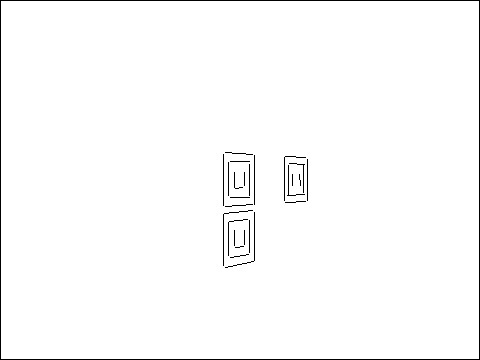
\includegraphics[scale=0.48]{figs_detection/limitesDeteccion/Caso4-LSD4.png}}
  \subfigure[Resultado de LSD para $r_y= 60 �$]{
    \includegraphics[scale=0.48]{figs_detection/limitesDeteccion/Caso4-LSD61.png}}
  \subfigure[Resultado de filtrado de segmentos para $r_y= -44 �$]{
    \includegraphics[scale=0.48]{figs_detection/limitesDeteccion/Caso4-LSDfilter9.png}}
  \subfigure[Resultado de filtrado de segmentos para $r_y= 52 �$]{
    \includegraphics[scale=0.48]{figs_detection/limitesDeteccion/Caso4-LSDfilter57.png}}
  \caption{L�mites para la rotaci�n m�xima y m�nima sobre el eje $y$.}
  \label{fig:benchmark_segmentos_ry}
\end{figure}

Las pruebas para los l�mites se resumen en la Tabla \ref{tab:limites}.
\begin{table}
\centering
\begin{tabular}{|c|c|c|c|} \hline
		& L�mite inferior & L�mite superior & Limita 	\\ \hline
Profundidad $z$ & $-$		  & $1575mm$	    & LSD	\\ \hline
Rotaci�n en $x$ & $-50�$	  & $54�$	    & LSD	\\ \hline
Rotaci�n en $y$ & $-44�$	  & $52�$	    & Filtrado	\\ \hline
\end{tabular}
\caption{Resumen de l�mites impuestos por los algoritmos de filtrado de segmentos y LSD para im�genes sint�ticas.}
\label{tab:limites}
\end{table}

\section{Resumen}
En este cap�tulo se comentaron algunos sistemas de Realidad Aumentada basados en marcadores planos como ARToolKit y ARTag. Se desarroll� el dise�o del Marcador QR utilizado para el proyecto y se definieron juegos de par�metros que permiten flexibilidad en la aplicaci�n de los mismos. Se desarrollaron los algoritmos para detecci�n de los marcadores dise�ados basados en un esquema de, en primer lugar, filtrado y agrupamiento de segmentos y en segundo lugar determinaci�n de correspondencias de sus esquinas. Se vi� que algunos de los par�metros de dise�o del marcador pueden ser modificados sin necesidad de modificar los algoritmos desarrollados. Finalmente se obtuvieron resultados de benchmark para los algoritmos de LSD y filtrado de segmentos mediante el uso de im�genes sint�ticas generadas con las herramientas de Benchmark. Se establecieron l�mites \emph{pseudo-te�ricos} para la profundidad del marcador, las rotaciones respecto al eje $x$ y respecto al eje $y$. Es importante destacar que estos l�mites son cotas raramente alcanzables por la aplicaci�n final ya que se utilizaron para eso im�genes sint�ticas sin ning�n tipo de ruido, cambios de iluminaci�n ni distorsi�n de c�mara.


\bibliographystyle{unsrt}   
\bibliography{encuadro}  
\end{document}
